% I seguenti commenti speciali impostano:
% 1. 
% 2. PDFLaTeX come motore di composizione;
% 3. tesi.tex come documento principale;
% 4. il controllo ortografico italiano per l'editor.

% !TEX encoding = UTF-8
% !TEX TS-program = pdflatex
% !TEX root = tesi.tex
% !TEX spellcheck = it-IT

% PDF/A filecontents
\RequirePackage{filecontents}
\begin{filecontents*}{\jobname.xmpdata}
  \Title{Document’s title}
  \Author{Author’s name}
  \Language{it-IT}
  \Subject{The abstract, or short description.}
  \Keywords{keyword1\sep keyword2\sep keyword3}
\end{filecontents*}

\documentclass[10pt,                    % corpo del font principale
               a4paper,                 % carta A4
               twoside,                 % impagina per fronte-retro
               openright,               % inizio capitoli a destra
               english,                 
               italian,                 
               ]{book}    

%**************************************************************
% Importazione package
%************************************************************** 

\PassOptionsToPackage{dvipsnames}{xcolor} % colori PDF/A

\usepackage{colorprofiles}

\usepackage[a-2b,mathxmp]{pdfx}[2018/12/22]
                                        % configurazione PDF/A
                                        % validare in https://www.pdf-online.com/osa/validate.aspx

%\usepackage{amsmath,amssymb,amsthm}    % matematica

\usepackage[T1]{fontenc}                % codifica dei font:
                                        % NOTA BENE! richiede una distribuzione *completa* di LaTeX

\usepackage[utf8]{inputenc}             % codifica di input; anche [latin1] va bene
                                        % NOTA BENE! va accordata con le preferenze dell'editor

\usepackage[english, italian]{babel}    % per scrivere in italiano e in inglese;
                                        % l'ultima lingua (l'italiano) risulta predefinita

\usepackage{bookmark}                   % segnalibri

\usepackage{caption}                    % didascalie

\usepackage{chngpage,calc}              % centra il frontespizio

\usepackage{csquotes}                   % gestisce automaticamente i caratteri (")

\usepackage{emptypage}                  % pagine vuote senza testatina e piede di pagina

\usepackage{epigraph}			% per epigrafi

\usepackage{eurosym}                    % simbolo dell'euro

%\usepackage{indentfirst}               % rientra il primo paragrafo di ogni sezione

\usepackage{graphicx}                   % immagini

\usepackage{hyperref}                   % collegamenti ipertestuali

\usepackage[binding=5mm]{layaureo}      % margini ottimizzati per l'A4; rilegatura di 5 mm

\usepackage{listings}                   % codici

\usepackage{microtype}                  % microtipografia

\usepackage{mparhack,fixltx2e,relsize}  % finezze tipografiche

\usepackage{nameref}                    % visualizza nome dei riferimenti                                      
\usepackage[font=small]{quoting}        % citazioni

\usepackage{subfig}                     % sottofigure, sottotabelle

\usepackage[italian]{varioref}          % riferimenti completi della pagina

\usepackage{booktabs}                   % tabelle                                       
\usepackage{tabularx}                   % tabelle di larghezza prefissata                                    
\usepackage{longtable}                  % tabelle su più pagine                                        
\usepackage{ltxtable}                   % tabelle su più pagine e adattabili in larghezza

\usepackage[toc, acronym]{glossaries}   % glossario
                                        % per includerlo nel documento bisogna:
                                        % 1. compilare una prima volta tesi.tex;
                                        % 2. eseguire: makeindex -s tesi.ist -t tesi.glg -o tesi.gls tesi.glo
                                        % 3. eseguire: makeindex -s tesi.ist -t tesi.alg -o tesi.acr tesi.acn
                                        % 4. compilare due volte tesi.tex.

\usepackage[backend=biber,style=verbose-ibid,hyperref,backref]{biblatex}
% eccellente pacchetto per la bibliografia; 
% produce uno stile di citazione autore-anno; 
% lo stile "numeric-comp" produce riferimenti numerici
% per includerlo nel documento bisogna:
% 1. compilare una prima volta tesi.tex;
% 2. eseguire: biber tesi
% 3. compilare ancora tesi.tex.

%**************************************************************
% file contenente le impostazioni della tesi
%**************************************************************

%**************************************************************
% Frontespizio
%**************************************************************

% Autore
\newcommand{\myName}{Giada Zuccolo}                                    
\newcommand{\myTitle}{Facebook Friend Requests' Analysis: development of tools for\\data collection and analysis}

% Tipo di tesi                   
\newcommand{\myDegree}{Tesi di laurea}

% Università             
\newcommand{\myUni}{Università degli Studi di Padova}

% Facoltà       
\newcommand{\myFaculty}{Corso di Laurea in Informatica}

% Dipartimento
\newcommand{\myDepartment}{Dipartimento di Matematica "Tullio Levi-Civita"}

% Titolo del relatore
\newcommand{\profTitle}{Prof.}

% Relatore
\newcommand{\myProf}{Mauro Conti}

% Luogo
\newcommand{\myLocation}{Padova}

% Anno accademico
\newcommand{\myAA}{2020-2021}

% Data discussione
\newcommand{\myTime}{Settembre 2021}


%**************************************************************
% Impostazioni di impaginazione
% see: http://wwwcdf.pd.infn.it/AppuntiLinux/a2547.htm
%**************************************************************

\setlength{\parindent}{14pt}   % larghezza rientro della prima riga
\setlength{\parskip}{0pt}   % distanza tra i paragrafi


%**************************************************************
% Impostazioni di biblatex
%**************************************************************
\bibliography{bibliografia} % database di biblatex 

\defbibheading{bibliography} {
    \cleardoublepage
    \phantomsection 
    \addcontentsline{toc}{chapter}{\bibname}
    \chapter*{\bibname\markboth{\bibname}{\bibname}}
}

\setlength\bibitemsep{1.5\itemsep} % spazio tra entry

\DeclareBibliographyCategory{opere}
\DeclareBibliographyCategory{web}

\addtocategory{opere}{womak:lean-thinking}
\addtocategory{web}{site:agile-manifesto}

\defbibheading{opere}{\section*{Riferimenti bibliografici}}
\defbibheading{web}{\section*{Siti Web consultati}}


%**************************************************************
% Impostazioni di caption
%**************************************************************
\captionsetup{
    tableposition=top,
    figureposition=bottom,
    font=small,
    format=hang,
    labelfont=bf
}

%**************************************************************
% Impostazioni di glossaries
%**************************************************************

%**************************************************************
% Acronimi
%**************************************************************
\renewcommand{\acronymname}{Acronimi e abbreviazioni}

\newacronym[description={\glslink{apig}{Application Program Interface}}]
    {api}{API}{Application Program Interface}

\newacronym[description={\glslink{umlg}{Unified Modeling Language}}]
    {uml}{UML}{Unified Modeling Language}

%**************************************************************
% Glossario
%**************************************************************
%\renewcommand{\glossaryname}{Glossario}

\newglossaryentry{apig}
{
    name=\glslink{api}{API},
    text=Application Program Interface,
    sort=api,
    description={in informatica con il termine \emph{Application Programming Interface API} (ing. interfaccia di programmazione di un'applicazione) si indica ogni insieme di procedure disponibili al programmatore, di solito raggruppate a formare un set di strumenti specifici per l'espletamento di un determinato compito all'interno di un certo programma. La finalità è ottenere un'astrazione, di solito tra l'hardware e il programmatore o tra software a basso e quello ad alto livello semplificando così il lavoro di programmazione}
}

\newglossaryentry{umlg}
{
    name=\glslink{uml}{UML},
    text=UML,
    sort=uml,
    description={in ingegneria del software \emph{UML, Unified Modeling Language} (ing. linguaggio di modellazione unificato) è un linguaggio di modellazione e specifica basato sul paradigma object-oriented. L'\emph{UML} svolge un'importantissima funzione di ``lingua franca'' nella comunità della progettazione e programmazione a oggetti. Gran parte della letteratura di settore usa tale linguaggio per descrivere soluzioni analitiche e progettuali in modo sintetico e comprensibile a un vasto pubblico}
}
 % database di termini
\makeglossaries


%**************************************************************
% Impostazioni di graphicx
%**************************************************************
\graphicspath{{immagini/}} % cartella dove sono riposte le immagini


%**************************************************************
% Impostazioni di hyperref
%**************************************************************
\hypersetup{
    %hyperfootnotes=false,
    %pdfpagelabels,
    %draft,	% = elimina tutti i link (utile per stampe in bianco e nero)
    colorlinks=true,
    linktocpage=false,
    pdfstartpage=1,
    pdfstartview=,
    % decommenta la riga seguente per avere link in nero (per esempio per la stampa in bianco e nero)
    %colorlinks=false, linktocpage=false, pdfborder={0 0 0}, pdfstartpage=1, pdfstartview=FitV,
    breaklinks=true,
    pdfpagemode=UseNone,
    pageanchor=true,
    pdfpagemode=UseOutlines,
    plainpages=false,
    bookmarksnumbered,
    bookmarksopen=true,
    bookmarksopenlevel=1,
    hypertexnames=true,
    pdfhighlight=/O,
    %nesting=true,
    %frenchlinks,
    urlcolor=webbrown,
    linkcolor=black,
    citecolor=webgreen,
    %pagecolor=RoyalBlue,
    %urlcolor=Black, linkcolor=Black, citecolor=Black, %pagecolor=Black,
    pdftitle={\myTitle},
    pdfauthor={\textcopyright\ \myName, \myUni, \myFaculty},
    pdfsubject={},
    pdfkeywords={},
    pdfcreator={pdfLaTeX},
    pdfproducer={LaTeX}
}

%**************************************************************
% Impostazioni di itemize
%**************************************************************
\renewcommand{\labelitemi}{$\ast$}

%\renewcommand{\labelitemi}{$\bullet$}
%\renewcommand{\labelitemii}{$\cdot$}
%\renewcommand{\labelitemiii}{$\diamond$}
%\renewcommand{\labelitemiv}{$\ast$}


%**************************************************************
% Impostazioni di listings
%**************************************************************
\lstset{
    language=[LaTeX]Tex,%C++,
    keywordstyle=\color{RoyalBlue}, %\bfseries,
    basicstyle=\small\ttfamily,
    %identifierstyle=\color{NavyBlue},
    commentstyle=\color{Green}\ttfamily,
    stringstyle=\rmfamily,
    numbers=none, %left,%
    numberstyle=\scriptsize, %\tiny
    stepnumber=5,
    numbersep=8pt,
    showstringspaces=false,
    breaklines=true,
    frameround=ftff,
    frame=single
} 


%**************************************************************
% Impostazioni di xcolor
%**************************************************************
\definecolor{webgreen}{rgb}{0,.5,0}
\definecolor{webbrown}{rgb}{.6,0,0}


%**************************************************************
% Altro
%**************************************************************

\newcommand{\omissis}{[\dots\negthinspace]} % produce [...]

% eccezioni all'algoritmo di sillabazione
\hyphenation
{
    ma-cro-istru-zio-ne
    gi-ral-din
}

\newcommand{\sectionname}{sezione}
\addto\captionsitalian{\renewcommand{\figurename}{Figura}
                       \renewcommand{\tablename}{Tabella}}

\newcommand{\glsfirstoccur}{\ap{{[g]}}}

\newcommand{\intro}[1]{\emph{\textsf{#1}}}

%**************************************************************
% Environment per ``rischi''
%**************************************************************
\newcounter{riskcounter}                % define a counter
\setcounter{riskcounter}{0}             % set the counter to some initial value

%%%% Parameters
% #1: Title
\newenvironment{risk}[1]{
    \refstepcounter{riskcounter}        % increment counter
    \par \noindent                      % start new paragraph
    \textbf{\arabic{riskcounter}. #1}   % display the title before the 
                                        % content of the environment is displayed 
}{
    \par\medskip
}

\newcommand{\riskname}{Rischio}

\newcommand{\riskdescription}[1]{\textbf{\\Descrizione:} #1.}

\newcommand{\risksolution}[1]{\textbf{\\Soluzione:} #1.}

%**************************************************************
% Environment per ``use case''
%**************************************************************
\newcounter{usecasecounter}             % define a counter
\setcounter{usecasecounter}{0}          % set the counter to some initial value

%%%% Parameters
% #1: ID
% #2: Nome
\newenvironment{usecase}[2]{
    \renewcommand{\theusecasecounter}{\usecasename #1}  % this is where the display of 
                       % the counter is overwritten/modified
    \refstepcounter{usecasecounter}             % increment counter
    \vspace{10pt}
    \par \noindent                              % start new paragraph
    {\large \textbf{\usecasename #1: #2}}       % display the title before the 
                                                % content of the environment is displayed 
    \medskip
}{
    \medskip
}

\newcommand{\usecasename}{UC}

\newcommand{\usecaseactors}[1]{\textbf{\\Attori Principali:} #1. \vspace{4pt}}
\newcommand{\usecasepre}[1]{\textbf{\\Precondizioni:} #1. \vspace{4pt}}
\newcommand{\usecasedesc}[1]{\textbf{\\Descrizione:} #1. \vspace{4pt}}
\newcommand{\usecasepost}[1]{\textbf{\\Postcondizioni:} #1. \vspace{4pt}}
\newcommand{\usecasealt}[1]{\textbf{\\Scenario Alternativo:} #1. \vspace{4pt}}

%**************************************************************
% Environment per ``namespace description''
%**************************************************************

\newenvironment{namespacedesc}{
    \vspace{10pt}
    \par \noindent          % start new paragraph
    \begin{description} 
}{
    \end{description}
    \medskip
}

\newcommand{\classdesc}[2]{\item[\textbf{#1:}] #2}
                     % file con le impostazioni personali

\begin{document}
%**************************************************************
% Materiale iniziale
%**************************************************************
\frontmatter
% !TEX encoding = UTF-8
% !TEX TS-program = pdflatex
% !TEX root = ../tesi.tex

%**************************************************************
% Frontespizio 
%**************************************************************
\begin{titlepage}

\begin{center}

\begin{LARGE}
\textbf{\myUni}\\
\end{LARGE}

\vspace{10pt}

\begin{Large}
\textsc{\myDepartment}\\
\end{Large}

\vspace{10pt}

\begin{large}
\textsc{\myFaculty}\\
\end{large}

\vspace{30pt}
\begin{figure}[htbp]
\begin{center}

\includegraphics[height=6cm]{logo-unipd}
\end{center}
\end{figure}
\vspace{20pt} 

\begin{LARGE}
\begin{center}
\textbf{\myTitle}\\
\end{center}
\end{LARGE}

\vspace{10pt} 

\begin{large}
\textsl{\myDegree}\\
\end{large}

\vspace{25pt} 

\begin{large}
\begin{flushleft}
\textit{Relatore}\\ 
\vspace{5pt} 
\profTitle \myProf\\
\end{flushleft}
\vspace{0pt} 
\begin{flushright}
\textit{Laureando}\\ 
\vspace{5pt} 
\myName
\end{flushright}
\end{large}
\begin{flushleft}
\textit{Correlatore}\\ 
\vspace{5pt} 
Pier Paolo Tricomi\\
\end{flushleft}
\vspace{12pt}
%\vfill

\line(1, 0){338} \\
\begin{normalsize}
\textsc{Anno Accademico \myAA}
\end{normalsize}

\end{center}
\end{titlepage} 
% !TEX encoding = UTF-8
% !TEX TS-program = pdflatex
% !TEX root = ../tesi.tex

%**************************************************************
% Colophon
%**************************************************************
\clearpage
\phantomsection
\thispagestyle{empty}

\hfill

\vfill

\noindent\myName: \textit{\myTitle,}
\myDegree,
\textcopyright\ \myTime.
% !TEX encoding = UTF-8
% !TEX TS-program = pdflatex
% !TEX root = ../tesi.tex

%**************************************************************
% Dedica
%**************************************************************
\cleardoublepage
\phantomsection
\thispagestyle{empty}
\pdfbookmark{Dedica}{Dedica}

\vspace*{3cm}

\begin{center}
Non come chi vince sempre\\ma come chi non si arrende mai. \\ \medskip
--- Frida Khalo    
\end{center}
%\begin{center}
%Sometimes it is the people who no one imagines anything of,\\who do the things no one can imagine. \\ \medskip
%--- Alan Turing, \textit{The Imitation Game}
%\end{center}

\medskip

%\begin{center}
%Dedicato a ...
%\end{center}

% !TEX encoding = UTF-8
% !TEX TS-program = pdflatex
% !TEX root = ../tesi.tex

%**************************************************************
% Sommario
%**************************************************************
\cleardoublepage
\phantomsection
\pdfbookmark{Sommario}{Sommario}
\begingroup
\let\clearpage\relax
\let\cleardoublepage\relax
\let\cleardoublepage\relax

\chapter*{Sommario}

Il presente documento descrive il lavoro svolto durante il periodo di stage, della durata di circa trecento ore, dal laureando Pinco Pallino presso l'azienda Azienda S.p.A.
Gli obbiettivi da raggiungere erano molteplici.\\
In primo luogo era richiesto lo sviluppo di ...
In secondo luogo era richiesta l'implementazione di un ... 
Tale framework permette di registrare gli eventi di un controllore programmabile, quali segnali applicati 
Terzo ed ultimo obbiettivo era l'integrazione ...

%\vfill
%
%\selectlanguage{english}
%\pdfbookmark{Abstract}{Abstract}
%\chapter*{Abstract}
%
%\selectlanguage{italian}

\endgroup			

\vfill


% !TEX encoding = UTF-8
% !TEX TS-program = pdflatex
% !TEX root = ../tesi.tex

%**************************************************************
% Ringraziamenti
%**************************************************************
\cleardoublepage
\phantomsection
\pdfbookmark{Ringraziamenti}{ringraziamenti}

%\begin{flushright}{
	%\slshape    
%	``Life is really simple, but we insist on making it complicated''} \\ 
%	\medskip
%    --- Confucius
%\end{flushright}


\bigskip

\begingroup
\let\clearpage\relax
\let\cleardoublepage\relax
\let\cleardoublepage\relax

\chapter*{Ringraziamenti}

\noindent Innanzitutto, vorrei esprimere la mia gratitudine al Prof. Mauro Conti, relatore della mia tesi, per aver creduto nelle mie idee ed avermi proposto di lavorare a questo progetto, ed insieme a PierPaolo, ringrazio per l'aiuto e il sostegno fornitomi durante il lavoro.\\

\noindent Voglio ringraziare più di tutti la mia famiglia per il costante sostegno e per essermi stati vicini in ogni momento, sia gioioso che difficoltoso, durante questi gli anni di studio.\\

\noindent Ringrazio poi i miei amici e compagni per questi anni passati insieme, da vicino e da lontano. In particolare ringrazio Sofia, per essere sempre stata una spalla e soprattutto un'amica su cui contare.\\

\noindent Ringrazio tutti i miei amici che sono qui a condividere questa gioia con me, soprattutto Clarissa, per l'appoggio che non mi ha fatto mai mancare e per la sua preziosa amicizia che per me è sempre stata un punto fermo.\\

\noindent \textit{Last but not least}, ringrazio con tutto il cuore Andrea, per avermi aiutata a vedere ed a tirare fuori sempre il meglio di me anche quando io non ci riuscivo, per avermi supportato (e sopportato) fin dal primo istante e per tutto l'amore che mi dimostra ogni giorno.\\
\bigskip

\noindent\textit{\myLocation, \myTime}
\hfill \myName

\endgroup


% !TEX encoding = UTF-8
% !TEX TS-program = pdflatex
% !TEX root = ../tesi.tex

%**************************************************************
% Indici
%**************************************************************
\cleardoublepage
\pdfbookmark{\contentsname}{tableofcontents}
\setcounter{tocdepth}{2}
\tableofcontents
%\markboth{\contentsname}{\contentsname} 
\clearpage

\begingroup 
    \let\clearpage\relax
    \let\cleardoublepage\relax
    \let\cleardoublepage\relax
    %*******************************************************
    % Elenco delle figure
    %*******************************************************    
    \phantomsection
    \pdfbookmark{\listfigurename}{lof}
    \listoffigures

    \vspace*{8ex}

    %*******************************************************
    % Elenco delle tabelle
    %*******************************************************
    \phantomsection
    \pdfbookmark{\listtablename}{lot}
    \listoftables
        
    \vspace*{8ex}
\endgroup

\cleardoublepage

\cleardoublepage

%**************************************************************
% Materiale principale
%**************************************************************
\mainmatter
% !TEX encoding = UTF-8
% !TEX TS-program = pdflatex
% !TEX root = ../tesi.tex

%**************************************************************
\chapter{Introduction}
\label{cap:introduction}
%**************************************************************
The exponential technological development and the internet have proliferated new criminally relevant conduct: new and more powerful IT tools have created new ways of committing a crime and have generated criminal phenomena.
\\For this reason, the area of primordial interest was the cybercriminal reality linked to the growing and hyperbolic development of the web and the technologies connected to it and how the types of crime (and criminals) and the most well-known and ordinary modus operandi have changed their physiognomy and have evolved with it.
\\Just think of online social networks and how they have an increasing impact on everyday life. Nowadays, social networks occupy a considerable part of daily life: they allow you to share links, photos, videos, thoughts, and to show your interest in some brands or companies. Many companies keep their customers updated through these channels, which can even be very useful for the growth of their customers, with shrewd and studied marketing skills.
In a more circumstantial reality, social networks allow you to stay in touch with friends near and far and favor the birth and development of relationships even with unknown users.
\\It's precisely in this context that the project takes shape. 
\\To start a relationship between two users, they must make contact, in some ways: generally or with a follow action (without some permissions) or with a friend request, where the user that receives the friend request has to accept (or not) the request to make contact with the other user. 
\\In the case of the social network par excellence, namely Facebook, a profile A asks for friendship to a profile B, who can choose whether to accept, leave pending or reject.
\\In fact, the person behind a virtual profile could be unknown: a person may have created a profile that does not belong to any real person but simulating its existence, to get in touch with some specific users.
\\This mechanism has led to the birth of online crime aimed at targeting specific people who, initially unaware, find themselves becoming \textit{victims}.\\From here, a first project idea was born: put the focus from the attacker's point of view and then create a tool to analyze a victim and suggest to the criminal a series of information be used to create a profile that the victim would more likely accept.

%\noindent Esempio di utilizzo di un termine nel glossario \\
%\gls{api}. \\

%\noindent Esempio di citazione in linea \\
%\cite{site:agile-manifesto}. \\

%\noindent Esempio di citazione nel pie' di pagina \\
%citazione\footcite{womak:lean-thinking} \\

%**************************************************************
\section{Organizzazione del testo}

\subsection{Contents}

\begin{description}
    \item[{\hyperref[cap:processi-metodologie]{Il secondo capitolo}}] descrive ...
    
    \item[{\hyperref[cap:descrizione-stage]{Il terzo capitolo}}] approfondisce ...
    
    \item[{\hyperref[cap:analisi-requisiti]{Il quarto capitolo}}] approfondisce ...
    
    \item[{\hyperref[cap:progettazione-codifica]{Il quinto capitolo}}] approfondisce ...
    
    \item[{\hyperref[cap:verifica-validazione]{Il sesto capitolo}}] approfondisce ...
    
    \item[{\hyperref[cap:conclusioni]{Nel settimo capitolo}}] descrive ...
\end{description}

\subsection{Typographic conventions}
Riguardo la stesura del testo, relativamente al documento sono state adottate le seguenti convenzioni tipografiche:
\begin{itemize}
	\item gli acronimi, le abbreviazioni e i termini ambigui o di uso non comune menzionati vengono definiti nel glossario, situato alla fine del presente documento;
	\item per la prima occorrenza dei termini riportati nel glossario viene utilizzata la seguente nomenclatura: \emph{parola}\glsfirstoccur;
	\item i termini in lingua straniera o facenti parti del gergo tecnico sono evidenziati con il carattere \emph{corsivo}.
\end{itemize}             % Introduzione
% !TEX encoding = UTF-8
% !TEX TS-program = pdflatex
% !TEX root = ../tesi.tex

%**************************************************************
\chapter{Description of the internship}
\label{cap:descrizione-stage}
%**************************************************************

In this chapter, there will explain the internship: the planning of work, the expected products, the objectives and methods of carrying out the activities\\

%**************************************************************
\section{A brief introduction to the project}
The general idea is studying the phenomenon of friend requests on Facebook, and how a profile with specific characteristics is accepted more easily by another profile with certain characteristics. \\
These characteristics, chosen after in-depth research in the literature, are defined by parameters (e.g. age, occupation, profile picture), which are divided into classes (e.g. age's class are defined by ranges, such as "age under 18", "age between 18 and 50 years old" or "over 50 years old").
\\Therefore, there will be developed specific tools capable to create a fake attacker profile with precise parameters and then send a friend request from this profile to more than one victim profile. \\The objective is to create a decided number of attacker profiles, based on the various combination of the parameters that we chose to analyze; then, all of these profiles must ask a friend request to a specific number of victim profiles which are categorized into configuration based on the various combination of the parameters that we have decided to analyze. In this way, we are sure that every type of attacker will ask at least one friend request to every type of victim. \\Consequently, an amount quantity of data will be collect and analyzed, in such a way as to be able to define a valid \textbf{model of acceptance}.
\\This is necessary to satisfy the concluding goal: define a functioning prototype for a final tool, which, after entering the URL of the victim, will take care of determining the characteristics that the attacker should include in his profile to be more likely accepted by the victim.
%**************************************************************
\section{Expected products}
The student had to keep track of the work done and the progress made against the expected progress day by day.\\
At the end of the internship period, the student had to produce a written report that keeps track of the work done and describes the results obtained, in particular:
\begin{enumerate}
	\item what has been learned from the study and research in literature; 
	\item the study, development, and execution of the tool for automating the search for a profile with certain characteristics;
	\item the study, development, and execution of the tool for the automation of the creation of an attacking profile with certain characteristics;
	\item the study, development, and execution of the tool for the automation of friend requests from a profile with certain characteristics to another profile with certain characteristics;	
	\item consecutive data collection; 
	\item a preliminary analysis of the collected data, aided by some tools developed ad hoc; 
	\item a prototype of a model of acceptance.
\end{enumerate}
%**************************************************************
\section{Objectives}
Now will be listed the objectives to achieve.
\begin{itemize}
\item implementation of the automatic search tool for people, given certain characteristics as input;
\item implementation of creation attacker profile tool, giving as input the characteristics that it must have;
\item implementation of the friend request tool from a profile to another profile, giving the necessary data as input;
\item preliminary analysis on previously collected data.
\end{itemize}

\subsection{Learning objectives expected}
During this internship the student will have the opportunity to deepen and put his knowledge into practice, in particular:
\begin{itemize}
	\item in the field of the automated management of browsers through the use of the Selenium framework;
	\item Python programming;
	\item tools and methodologies for data collection; 
	\item statistical techniques and tools for the study and analysis of the collected data.
\end{itemize}
%**************************************************************
%\section{Methods of carrying out activities}
%Most of the internship activity was carried out in smart working, due to the health emergency due to Covid-19.
%However, the contacts with the proposing tutor took place weekly with an interview, verifying the progress and any discrepancies with the work plan, to refine the objectives and update the work plan.
%The student was required to work 8 hours a day from Monday to Friday, approximately from 8.30 to 12.30 and from 14.30 to 18.30, for a total of 320 hours.
%**************************************************************
%\section{Planning of the activities}             % Processi
% !TEX encoding = UTF-8
% !TEX TS-program = pdflatex
% !TEX root = ../tesi.tex

%**************************************************************
\chapter{Descrizione dello stage}
\label{cap:descrizione-stage}
%**************************************************************

\intro{Breve introduzione al capitolo}\\

%**************************************************************
\section{Introduzione al progetto}

%**************************************************************
\section{Analisi preventiva dei rischi}

Durante la fase di analisi iniziale sono stati individuati alcuni possibili rischi a cui si potrà andare incontro.
Si è quindi proceduto a elaborare delle possibili soluzioni per far fronte a tali rischi.\\

\begin{risk}{Performance del simulatore hardware}
    \riskdescription{le performance del simulatore hardware e la comunicazione con questo potrebbero risultare lenti o non abbastanza buoni da causare il fallimento dei test}
    \risksolution{coinvolgimento del responsabile a capo del progetto relativo il simulatore hardware}
    \label{risk:hardware-simulator} 
\end{risk}

%**************************************************************
\section{Requisiti e obiettivi}


%**************************************************************
\section{Pianificazione}             % Kick-Off
% !TEX encoding = UTF-8
% !TEX TS-program = pdflatex
% !TEX root = ../tesi.tex

%**************************************************************
% !TEX encoding = UTF-8
% !TEX TS-program = pdflatex
% !TEX root = ../tesi.tex

%**************************************************************
\chapter{Literature search}
\label{cap:literature-search}
%**************************************************************
The research in the literature and the study of founded projects was useful for the knowledge of the possible areas and above all, it was necessary to verify that no other project had as a focal point the attacker who wants to hit a specific victim and must make sure to be accepted as a possible friend. Furthermore, these papers were useful to delineate the parameters from which to structure the attackers' and victims' profiles.
\section{List of papers}
Many papers are dealing with this social network, each of which opened to the perspective of many other projects. The most important and useful papers found in the great research phase are now shown and discussed:
\begin{enumerate}
	\item 
	\textsc{INVESTIGATIVE TECHNIQUES IN THE DIGITAL AGE - CYBERCRIME AND CRIMINAL PROFILING} \parencite{site:paper1}
	\par In this paper, it is made clear how cyberspace offers the possibility of carrying out illicit acts with the perception of going unpunished, showing the new various types of crimes such as cyberstalking, cyberbullying, online sexual offenses, etc. Cyberspace has allowed the criminal to evolve the techniques and approaches to the victim, so much so that it is not always immediately obvious that the intentions of one account towards another can be malicious. This new world, moreover, places investigators to consider the crime scene differently: a crime born of a victim's approach on the web places the computer itself as a victim or as a witness, but above all as a crime scene and therefore as a space to be analyzed. that could help (or penalize?) the investigators. 
	
	\item 
	\textsc{ONLINE SOCIAL NETWORKS AS SUPPORTING EVIDENCE: A DIGITAL FORENSIC INVESTIGATION MODEL AND ITS APPLICATION DESIGN} \parencite{site:paper2}
	\par This paper states that digital crime investigations are performed without adequate guidelines, as there isn't a consistent standard and model, only a set of procedures and tools, and above all, there is no model built specifically for social networks. This paper, therefore, proposes a standard survey model to be used for social networks, incorporating existing traditional frameworks and strategies.. 
	\newpage
	\item
	\textsc{INTEGRO: LEVERAGING VICTIM PREDICTION FOR ROBUST FAKE ACCOUNT DETECTION IN ONLINE SOCIAL NETWORKS} \parencite{site:paper3}
	\par The \textit{Integro} project is a scalable defense system that helps Online Social Networks detect fake accounts using a meaningful user classification scheme. This paper, in addition to providing an explanation of how \textit{Integro} works, provides interesting explanations on the behaviors that differentiate the attacker and the victim.
	
	\item
	\textsc{SOCIALSPY: BROWSING (SUPPOSEDLY) HIDDEN INFORMATION IN ONLINE SOCIAL NETWORKS} \parencite{site:paper4}
	\par This paper highlights how current privacy settings in social networks are not as effective as users might think, focusing on Facebook. It shows how easy it is to retrieve information that a user thinks they have set as private.
	
	\item 
	\textsc{EVALUATION OF THE LIKELIHOOD OF FRIEND REQUEST ACCEPTANCE IN ONLINE SOCIAL NETWORKS} \parencite{site:paper5}
	\par This paper explains how Online Social Networks users often run into breaches or security issues due to rash acceptance of the friend request, which can lead to the disclosure of personal information and vulnerability to an attack. The document proposes a method to evaluate the probability of becoming a friend having defined a model data: a future friend and incoming friend requests are evaluated with reference to this model which takes into account the attributes (such as common interests) and behavioral properties (such as seat frequency).
	
	\item
	\textsc{CAN FRIENDS BE TRUSTED? EXPLORING PRIVACY IN ONLINE SOCIAL NETWORKS} \parencite{site:paper6}
	\par This article presents a case study describing the privacy and trust inside a small population of online social network users. Taking Facebook as a reference, the frequency with which people are willing to disclose personal data to an unknown online user was determined. While most of the users sampled did not share sensitive information when requested by the stranger, it turned out that several users were willing to divulge personal details to a stranger if there is a mutual friend.	
	
	\item 
	\textsc{TO BEFRIEND OR NOT: A MODEL OF FRIEND REQUEST ACCEPTANCE} \parencite{site:paper7}
	\label{cap:to-be-friend}
	\par This paper was the most useful, as it provided a valid model for the choice of parameters: it explains how a friend request acceptance model was developed that explains how various factors influence user acceptance behavior. This paper highlighted how there are 4 decision-making factors to which a user appeals when he has to accept a friend request, in particular, \textit{<<friendship factors>>}, i.e., all the visible aspects of the profile (name, gender, profile picture, city of origin, residence, school, mutual friends, interests, etc.); \textit{<<privacy factors>>}, dictated by a personal concern of a user and/or awareness of her, perhaps also due to personal experiences or friends; \textit{<<environmental factors>>}, when friend requests are accepted without actually considering those who arrive due to lack of concentration and/or time to check; in the end \textit{<<capacity of interface>>}, that means that some types of users spend a lot of time to understand what kind of person has asked them for friendship, with careful evaluation of all the information and photos of that profile, until sending a private message. Some users keep the friend request pending and reserve the right to check the profile occasionally, to see changes within it.
\end{enumerate}

\section{Summary and starting points}
Continuing with the research, the focus has increasingly focused on the type of projects that could have turned out to be similar to the idea of putting oneself on the side of the attacker who wants to hit a specific victim and must ensure that he is accepted as a possible friend. All the papers found were useful to outline the parameters from which to start to structure the attacking and victim profiles.
\par \noindent In the next chapters, the parameters and the development choices will be motivated based on the aspects that the study in the literature has allowed evaluating.             % Concept Preview
% !TEX encoding = UTF-8
% !TEX TS-program = pdflatex
% !TEX root = ../tesi.tex

%**************************************************************
\chapter{Structure design}
\label{cap:structure-design}
%**************************************************************

The attacker knows that it is not easy to be accepted by his victim and, for this reason, he wants to understand what choices he must take to create the best profile possible to be accepted without too much delay by the victim. Therefore, the parameters must be defined based on the victim, to be accepted with greater possibility.
\par \noindent Thanks to the study of some specific papers mentioned above and thinking about how much to deepen the search for the best profile, in this chapter will be define and explain the chosen parameters. Then, from the parameters, the consequent profiles configurations will be shown.

%**************************************************************
\section{Project guidelines and the chosen parameters}
The definition of the parameters was conditioned by the degree of depth that the project wants to achieve: clearly more parameters lead to a greater number of profile configurations, but the data collection must be more in-depth and on a large scale. Furthermore, Facebook does not check that the date of birth that a user enters at the time of registration is true (therefore that he is really the age he claims to be) but that it only checks if it is valid for its standards (if it is at least 13 years old and if it's not existent like February 30th). This means that a person could enter data that is valid for Facebook but not true in reality. Assuming that there is always a real person behind a profile, untrue data would lead to an invalid analysis. Therefore, the parameters chosen are parameters that when registering on Facebook, a person would be required to be honest.\par \noindent 
It should be underlined how the resulting configuration of the profiles can be considered as the starting point: in the future the study could be deepened, adding other parameters, but this can be done by taking this as the starting configuration.

\subsection{First parameter: gender}
Gender is almost the most relevant factor, so much that most of the time is the decisive one. If looking at the profile's name, the gender is not clear, an user can check the bio of this profile. In fact, in the bio, the correspondent label of the gender will specify because a person who wants to register on Facebook must declare it and could be ``woman'', ``man'' or ``custom option'' where a user can set its pronouns. \par \noindent 
By the way, many papers of those cited report that a friend request from a female user profile is accepted easier than a friend request from a man user profile, regardless of the gender of the profile that receives it (an example of paper that report this statement is <<\textit{To be friend or not: a model of friend request acceptance}>>\parencite{site:paper7}, discussed on page \pageref{cap:to-be-friend}).
\subsubsection*{Classes}
The parameter \texttt{gender} $ \in \{$\texttt{female, male}$\}$, where: 
\begin{itemize}
	\item \texttt{female/F}, if the victim's profile user declares to be a \textit{female};
	\item \texttt{male/M}, if the victim's profile user declares to be a \textit{male}.
\end{itemize}
\subsection{Second parameter: image profile}
\label{cap:alt-technology}
The profile picture is the first thing, along with the name, a user sees when they have a friend request. As reported in some above-mentioned papers, the profile image already serves to give an idea of the person who is asking for friendship, because it shows some details that do not need to be checked (such as gender or an indicative age range).
A profile with a hidden or fake image (eg. a landscape) is more mysterious in the eyes of a user who receives the friend request, beacuse the real person behind this profile is not clearly identifiable. Therefore, the main idea is to verify the presence of at least one person in the profile picture and classify the user profiles based on the outcome of this verification.\par \noindent 
Facebook uses a technology that allows recognizing the profile image's content (faces, objects, ...) \parencite{site:alt-text} , and automatically creating a description that will be enclosed in the \texttt{alt} tag. 
The presence of one or more people (and occasionally other details about the panorama and/or some objects present) is always specified within the \texttt{alt} tag. On the other hand, if the image is fictional (cartoons, drawings, etc.) or is an image without a person (eg. landscapes), the \texttt{alt} tag contains ``\texttt{No description of the photo available}``. This technology has been exploited to classify each victim's profile picture.
\subsubsection*{Classes}
The parameter \texttt{real\_img} $ \in \{$\texttt{true,false}$\}$, where: 
\begin{itemize}
	\item \texttt{true}, if in \texttt{alt} tag reported the presence of one or more people;
	\item \texttt{false}, if in \texttt{alt} tag not reported the presence of one or more people;
\end{itemize}
\subsection{Third parameter: age} 
\label{cap:age-parameter}
Age is a very relevant factor. From the literature, it appears to be one of the first factors that a user who receives a friendship goes to check the profile from which the friend request started, if the age is not deducible from the image profile. 
The more similar age, the more likely it is that the friend request will be accepted. A person who wants to register on Facebook, must declare a real birth date (and must be at least 13 years old) and, once the profile has been created, can choose whether to make the date public or not. Some profiles publish only the month and day, other profiles only the year, others the complete date, others hide everything.\par \noindent To classify profile user's age, the date of birth that it reports will be taken, and the age will be calculated based on the current year, so as to be able to assign to this profile its membership class.
\subsubsection*{Classes}
Age is classified into 3 ranges, so the parameter \texttt{age\_range} $ \in \{2,3,4\}$, where: 
\begin{itemize}
	\item \texttt{2}, if the age victim's profile user is between 18 and 50 years;
	\item \texttt{3}, if the age victim's profile user is greater than 50 years;
	\item \texttt{4}, if the age victim's profile user is hidden;
\end{itemize}

\section{Parameters' configuration for creating profiles}
\label{cap:table-configuration}
To delineate the types of profiles (the same for both victims and attackers) it was necessary to define profile categories, which are nothing more than the combinations of all the various parameters.\par \noindent 
In this case study, the parameters that will be configured are:
\begin{enumerate}
	\item \texttt{gender} $ \in \{$\texttt{female, male}$\}$;
	\item \texttt{real\_img} $ \in \{$\texttt{true,false}$\}$;
	\item \texttt{age\_range} $ \in \{2,3,4\}$.
\end{enumerate}
Combining all various parameters with possible values, there are $12$ profiles and $12 \cdot 12 = 144$ possible attack combinations. All the various resulting configurations are now shown in Table \ref{table:configuration}:
\begin{table}[h!]
\begin{center}
	\begin{tabular}{ |c|c|c|c| } 
		\hline 
		\cellcolor[HTML]{b0d7ff} \texttt{gender} & 
		\cellcolor[HTML]{b0d7ff} \texttt{real\_img} & 
		\cellcolor[HTML]{b0d7ff} \texttt{age\_range} &
		\cellcolor[HTML]{b0d7ff} \textsc{label}	\\
		\hline 
		\texttt{female}	&	\texttt{true}	&	\textsc{2}	
		&	\cellcolor[HTML]{e6f2ff} \texttt{FT2}\\	 
		\hline
		\texttt{female}	&	\texttt{true}	&	\textsc{3}	
		&\cellcolor[HTML]{e6f2ff} \texttt{FT3}\\	 
		\hline
		\texttt{female}	&	\texttt{true}	&	\textsc{4}	
		& \cellcolor[HTML]{e6f2ff} \texttt{FT4}\\	 
		\hline
		\texttt{female}	&	\texttt{false}	&	\textsc{2}	
		& \cellcolor[HTML]{e6f2ff} \texttt{FF2}\\	 
		\hline
		\texttt{female}	&	\texttt{false}	&	\textsc{3}	
		& \cellcolor[HTML]{e6f2ff} \texttt{FF3}\\
		\hline
		\texttt{female}	&	\texttt{false}	&	\textsc{4}	
		& \cellcolor[HTML]{e6f2ff} \texttt{FF4}\\
		\hline 	
		\texttt{male}	&	\texttt{true}	&	\textsc{2}	
		& \cellcolor[HTML]{e6f2ff} \texttt{MT2}\\
		\hline
		\texttt{male}	&	\texttt{true}	&	\textsc{3}	
		& \cellcolor[HTML]{e6f2ff} \texttt{MT3}\\	 
		\hline
		\texttt{male}	&	\texttt{true}	&	\textsc{4}	
		& \cellcolor[HTML]{e6f2ff} \texttt{MT4}\\
		\hline
		\texttt{male}	&	\texttt{false}	&	\textsc{2}	
		& \cellcolor[HTML]{e6f2ff} \texttt{MF2}\\
		\hline
		\texttt{male}	&	\texttt{false}	&	\textsc{3}	
		& \cellcolor[HTML]{e6f2ff} \texttt{MF3}\\
		\hline
		\texttt{male}	&	\texttt{false}	&	\textsc{4}	
		& \cellcolor[HTML]{e6f2ff} \texttt{MF4}\\
		\hline 	 	 	 	 	
	\end{tabular}
	\caption{Profile configurations, identified by a label, based on the combinations of the parameters which are gender, age and profile picture.}
	\label{table:configuration}
\end{center}
\end{table}
\subsection*{The label}
As can be seen from the table above, each type of profile is classified with a \textit{label}. The label is the union of the actual value assumed by the parameters in that particular circumstance: the first character identifies the gender (``\texttt{F}'' in the case of ``\texttt{female}``, ``\texttt{M}'' in the case of ``\texttt{male}``), the second character indicates the value of the ``\texttt{real\_img}'' parameter (``\texttt{T}'' in case it is ``\texttt{true}``, ``\texttt{F}'' in case it is ``\texttt{false}``) and the last character is the numeric value that indicates the age range (it can be ``\texttt{2}``, ``\texttt{3}'' or ``\texttt{4}``). All \textit{victim profiles} are classified with these labels. In fact, each collected \textit{victim profile} is labeled into one of these $12$ categories.\par \noindent However, as regards the \textit{attackers} profiles, they will be created starting from these configurations and in an automated way with the help of the tool called \texttt{create-profile.py} (details in the Chapter \ref{cap:tool-create}). Furthermore, if attackers and victims have the same label it could be brought to create confusion in the second phase of the organization of the attack combinations. For this reason, the attackers' profiles are identified with an identifying code ``\texttt{PF-}\textit{n}'' where \textit{n} is an increasing identification number assigned when the profile is created. 

\section{Development planning}
Development takes place in 4 consecutive phases:
\begin{enumerate}
	\item  create the 12 attacker profiles;
	\item  collect victim profiles and classify each of them in its category;
	\item  each attacker profile will require the friendship of 3 victim profiles for each category (details in Chapter \ref{cap:number-friend-req});
	\item  analysis of the collected data (how many profiles have accepted the friendship, which category they belong to and which category the respective attacker belongs to, ...).		
\end{enumerate}

\section{System architecture}
The Figure \ref{fig:system-arc} on the following page graphically shows the general architecture of the system:
\begin{description}
	\item[blue rectangles] indicate the possible actions that can be performed.\par \noindent They are listed vertically to show the chronological sense of their execution.
	\item[green rectangles] indicate the developed tools.\par \noindent Note that the \texttt{round-add.py} tool is surrounded by a \textit{red rectangle with a dashed border} to indicate that it must be run only once and before the first run of the \texttt{add-friend.py} tool. \par \noindent Furthermore, the \textit{green arrows} that connect one tool to another, indicate a chronological order in which the tools must be executed each time.
	\item[yellow rectangles] indicate the resulting datasets after running that tool.\par \noindent These datasets can be used for subsequent actions. In fact, note the \textit{orange arrows}: they indicate which specific dataset is required in order to run the tool to which it is connected.
\end{description}
\newpage
\begin{figure}[h]
	\caption{System architecture of the tools}
\begin{center}
	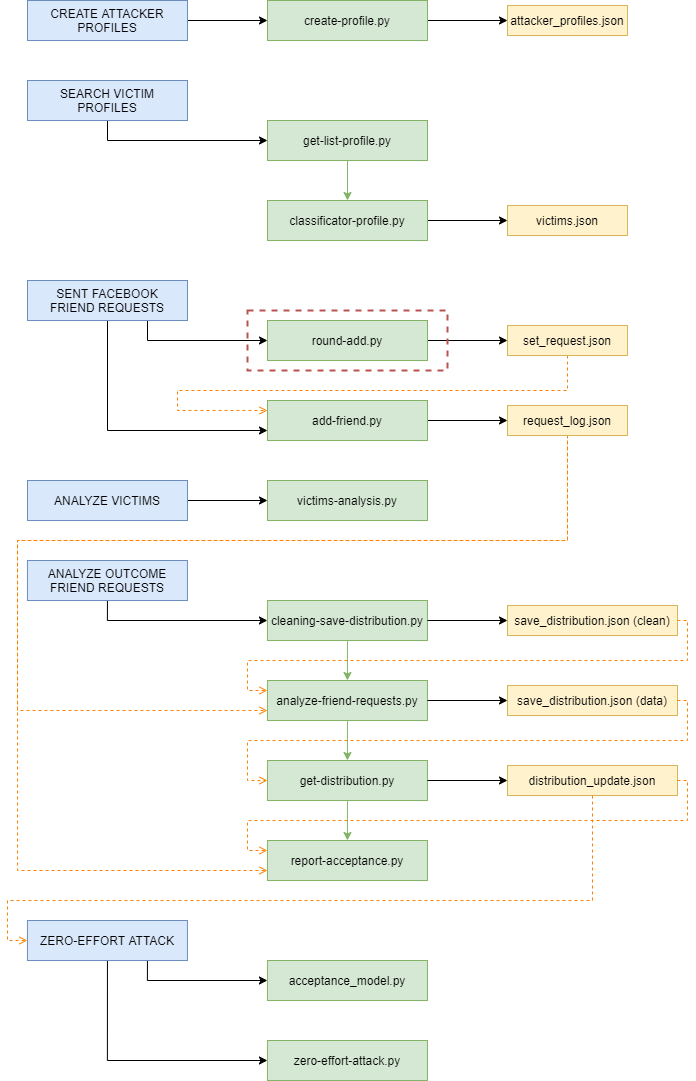
\includegraphics[width=13cm]{immagini/architecture-system.png} 
\end{center}
\label{fig:system-arc}
\end{figure}
             % Product Prototype
% !TEX encoding = UTF-8
% !TEX TS-program = pdflatex
% !TEX root = ../tesi.tex

%**************************************************************
\chapter{Development of the tools}
\label{cap:tools}
In this chapter the study behind the development of every single created tool will be explain, and technical details about implementation.
%**************************************************************

\section{Tool for automated create of attacker's profile}
This section reports the study and development process of the tool for the automated creation of an attacker profile.

\subsection{The tool: \texttt{create-profile.py}}
\label{cap:tool-create}
The attacker profiles were created from the various profile category configurations identified in chapter \ref{cap:table-configuration}. The process is automated, that is, using a tool, called "\texttt{create-profile.py}", which after requesting specific values as input, responds in output with a complete card of the attacking profile's personal data.
\\\\\noindent The tool, run from the terminal, requires as input:
\begin{itemize}
	\item \texttt{cod\_id},\\an identification code to identify the profile in a simpler way (with this parameter, \texttt{PF-}\textit{n} will be created, where \textit{n} is this \texttt{cod\_id}).\\Accepted values: numeric parameter (\texttt{int});
	
	\item \texttt{gender},\\i.e. the gender of the attacker\\Accepted values: string parameter $s$, with $s \in \{$\texttt{female, male}$\}$;
	
	\item \texttt{real\_img},\\boolean value for the type of image profile the attacker must have.\\Accepted values: boolean parameter (\texttt{true} or \texttt{false});
	
	\item \texttt{age},\\i.e. the age of the attacker.\\Accepted values: numeric parameter (\texttt{int});
	
	\item \texttt{agehide},\\boolean value for whether the age will be visible in the profile or not.\\Accepted values: boolean parameter (\texttt{true} or \texttt{false}).
\end{itemize}
\noindent \\ Moreover, the tool use datasets (created ad hoc) to generate a most complete and realistic profile possible:
\begin{itemize}
	\item \texttt{dataset-name.json}, to randomly assign the name to the profile, based on the input \texttt{gender} parameter; this dataset is formed with the most common Italian names, both male and female, more than 100 for each.
	\item \texttt{dataset-surname.json}, to randomly assign the surname to the profile; this dataset is formed with the 100 most common Italian surnames.
	\item \texttt{dataset-city.json}, containing the list of Italian provinces to randomly assign the city of residence to the profile;
	\item \texttt{dataset-occupation.json}, to randomly assign the job occupation to the profile;
\end{itemize} 

\subsection{Develop of the tools}
First of all, using \texttt{dataset-name.json}, a random name is extract and assign to the profile, based on the input \texttt{gender} parameter.
\\Same thing for the surname where, using \texttt{dataset-surname.json}, a random surname is extract and assign to the profile.
\\\\After that, \texttt{real\_img} parameter and \texttt{gender} parameter will be check, and, the label to identify the attacker the label begins to be created. 
\\\\With the \texttt{age} parameter, the tool will then create an appropriate date of birth to be entered in the Facebook profile, both in the case \texttt{agehide} parameter is "\texttt{true}" or "\texttt{false}", because to register on Facebook it is necessary to enter a date of valid birth. \\With the correct age range, the last character of the label could be set now, so the \textit{label} is created.
\\\\Despite \texttt{residence} and \texttt{occupation} are superfluous parameters fot this case of study, to make each attacker profile more complete and realistic, actual values were nevertheless entered, which obviously were not valued in the analysis for research purposes.
\\\\About \texttt{occupation}, a minimum of control has been included, to make it consistent with age and leaving aside some special cases: each profile under the age of 18 will have a "\texttt{Studentessa}" or "\texttt{Studente}", while each profile over the age of 65 will have "\texttt{Pensionata}" or "\texttt{Pensionato}" as occupation.
\\\\About \texttt{residence}, an attempt was made to scatter the various attacker profiles throughout the Italian peninsula. This was done in order not to risk having more attacker profiles in too close areas.
\\\\Afterwards, the tool uses the temporary fake email generator service (at \url{https://emailfake.com/} site) to create the fake email with which this profile will then log into Facebook. The username of the email is made up of \texttt{nome.cognome.age}, for each profile. The tool will go to the temporary false email generator site, enter the username created in the appropriate input section and then save the complete email with the random domain that the site will propose.
\\\\Consequently, the tool generates a password of 6 characters, formed by an uppercase letter, 4 lowercase letters, 2 numbers, and a special character, to use to log into Facebook.
\\\\In the end, the tool generate the identification \textit{code} with the \texttt{cod\_id} (for example \texttt{PF-3}), and save the data in the dataset \texttt{attacker\_profiles.json}.

\subsection{Create Facebook accounts}
Originally, one idea was to create the Facebook account in an automated way, using a tool developed ad hoc.
\\Unfortunately, however, in the study phase, it was seen how the social network applies very strict policies that often constrained the creation of these profiles.
\\First of all, it required to enter a code that he would send by email and occasionally forced the resolution of a ReCAPTCHA to continue. \\Sometimes the email with the code not arrived, so the procedure broke up and the profile was blocked. 
\\In other cases, Facebook continued to ask to resolve ReCAPTCHAs, even though they were always resolved correctly, and, after a while, the profile was blocked.
\\\\Therefore, the creation is done manually, but, despite this, there were still some significant problems: in fact, many profiles, after entering the initial data were immediately blocked and could only be unlocked by entering a mobile number.
\\\\So it was necessary frequently changing browser, connection, device, operating system, and even site for the generation of temporary emails. \\To avoid running into further blocks, the profiles were created gradually, that is, days apart from each other.
\\\\Once created, each profile was included in numerous Facebook groups of different genres (reading, music, sports, etc.) and occasionally some content was shared in their personal profile.
\\\\Furthermore it's important to underline that some profiles with \texttt{real\_img} parameter set as \texttt{false} are minors, although in chapter 5.1.3 it can be seen how the 3 age ranges only consider adult people.\\This was done because the age of these profiles, as evidenced by the corresponding \textit{label}, is not visible to the victim profiles who find the friend request, as the age is hidden.
\\\\The last step concerns the profile picture. It is necessary to specify that the profile pictures where the \texttt{real\_img} parameter is set to \texttt{true} are not of real people, as they were fished from this site: \url{https://thispersondoesnotexist.com/}. It generates a realistic picture of a person every time the page is refreshed, using artificial intelligence. So, the profile pictures were obviously chosen after creating every single attacker profile with the tool, because it was necessary to be consistent with the age of the profile user.
\\In the end, the profile pictures where the \texttt{real\_img} parameter is set to \texttt{false} were chosen looking random images in Google Images.
\\\\The 12 attacking profiles that have been generated are now reported.\\
%\begin{table}[h]
%	\centering

\begin{tabular}[c]{ |c|c|m{1.5cm}|c|c|c|c|m{1.85cm}| } 
	\hline
	\cellcolor[HTML]{b0d7ff}\textsc{cod} & 
	\cellcolor[HTML]{b0d7ff}\textsc{label} & 
	\multicolumn{1}{|c|}{\cellcolor[HTML]{b0d7ff}\textsc{img}}&
	\cellcolor[HTML]{b0d7ff}\textsc{name} & 
	\cellcolor[HTML]{b0d7ff}\textsc{surname} &
	\cellcolor[HTML]{b0d7ff}\textsc{age} &
	\cellcolor[HTML]{b0d7ff}\textsc{residence}	&
	\cellcolor[HTML]{b0d7ff}\textsc{occupation}	\\
	%\cellcolor[HTML]{e6f2ff}
	\hline 
	\cellcolor[HTML]{b0d7ff}\texttt{PF-11}&\cellcolor[HTML]{e6f2ff}\texttt{FT2}&	
	\vspace{.15cm}
	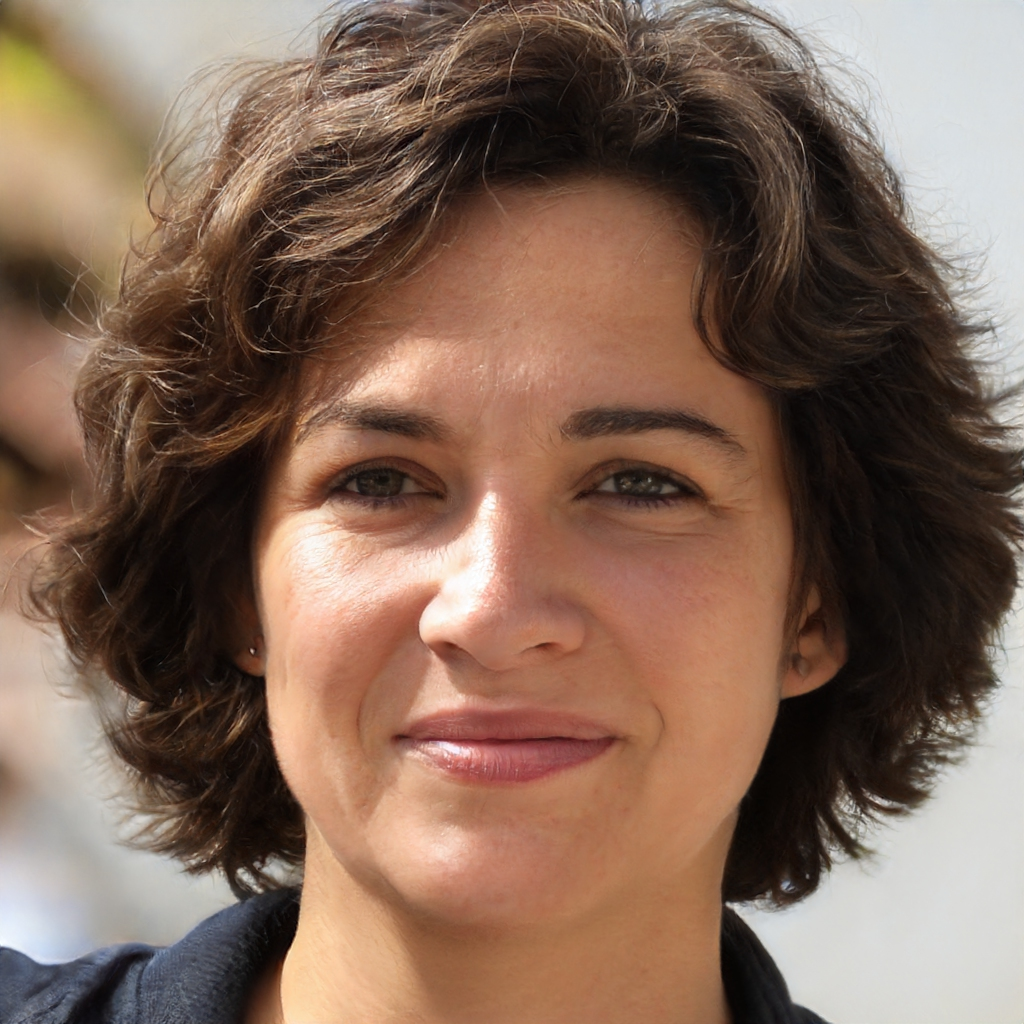
\includegraphics[height=1.5cm]{immagini/FT2.jpg}			
	&Federica&Grasso&38&Milano&Agente \newline Assicurativo\\	
	\hline
	\cellcolor[HTML]{b0d7ff}\texttt{PF-9}&\cellcolor[HTML]{e6f2ff}\texttt{FT3}&	
	\vspace{.15cm}		
	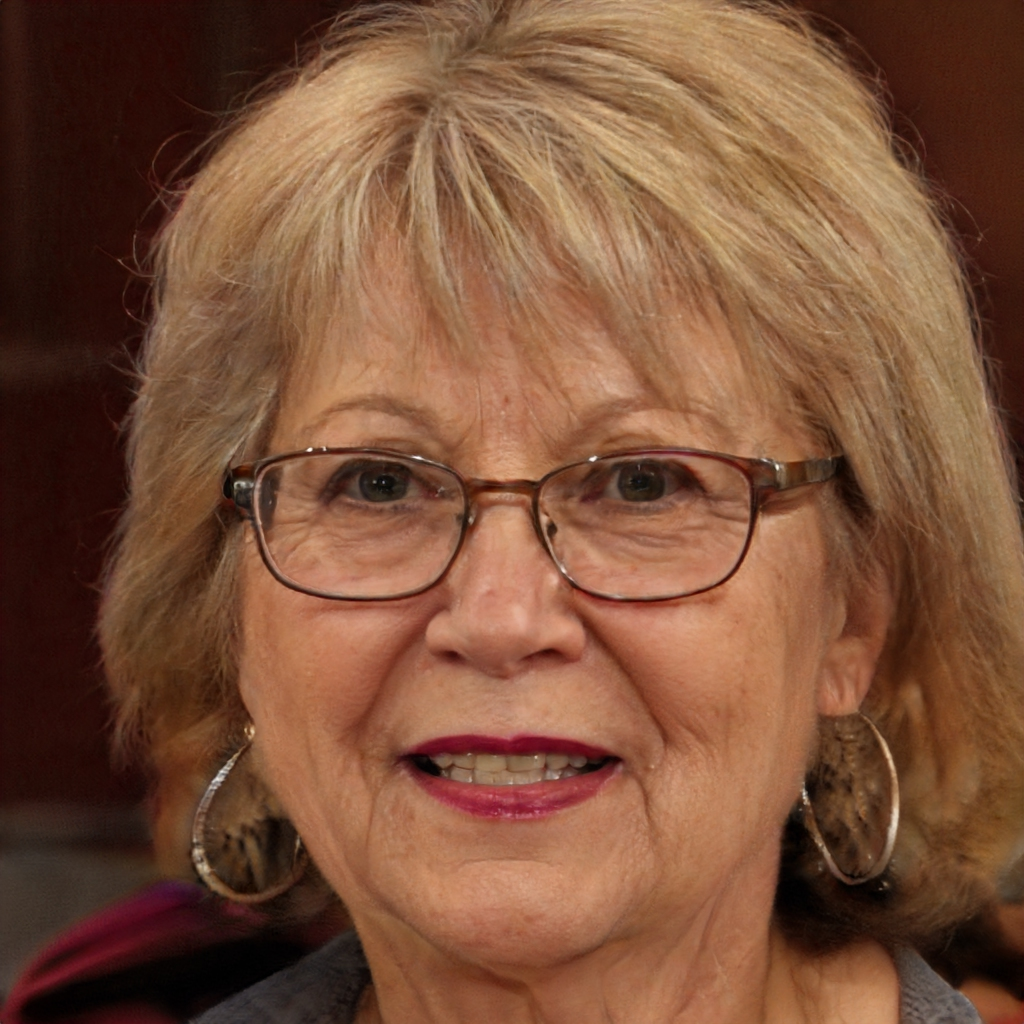
\includegraphics[height=1.5cm]{immagini/FT3.jpg}
	&Giulia&Moro&72&Vercelli&Pensionata\\	 
	\hline
	\cellcolor[HTML]{b0d7ff}\texttt{PF-6}&\cellcolor[HTML]{e6f2ff}\texttt{FT4}&	
	\vspace{.15cm}
	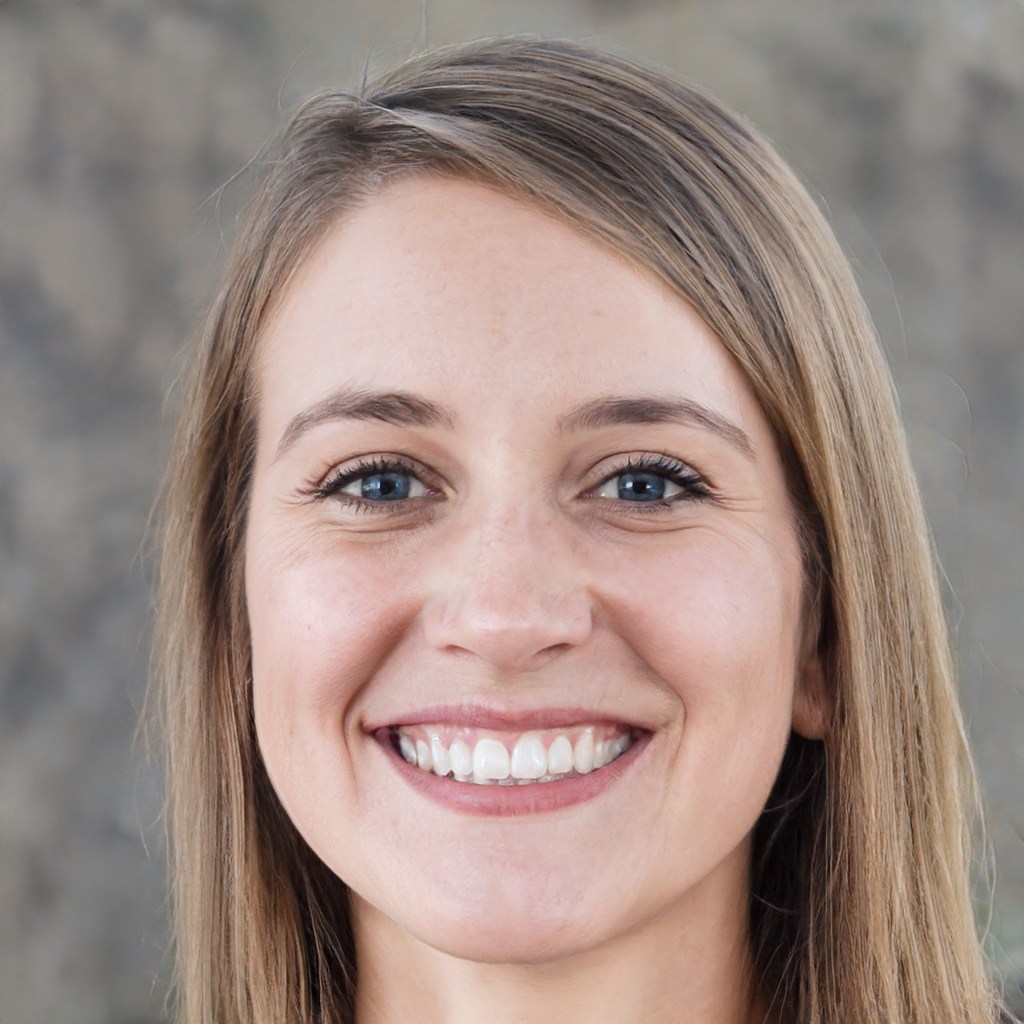
\includegraphics[height=1.5cm]{immagini/FT4.jpg}
	&Giulia&Ferrari&32&Palermo&Istruttrice di Yoga\\ 
	\hline
	\cellcolor[HTML]{b0d7ff}\texttt{PF-8}&\cellcolor[HTML]{e6f2ff}\texttt{FF2}&	
	\vspace{.15cm}
	
\includegraphics[height=1.5cm]{immagini/FF2.png}
	&Ilaria&Riva&26&Verona&Stilista\\	 
	\hline
	\cellcolor[HTML]{b0d7ff}\texttt{PF-10}&\cellcolor[HTML]{e6f2ff}\texttt{FF3}&	
	\vspace{.15cm}
	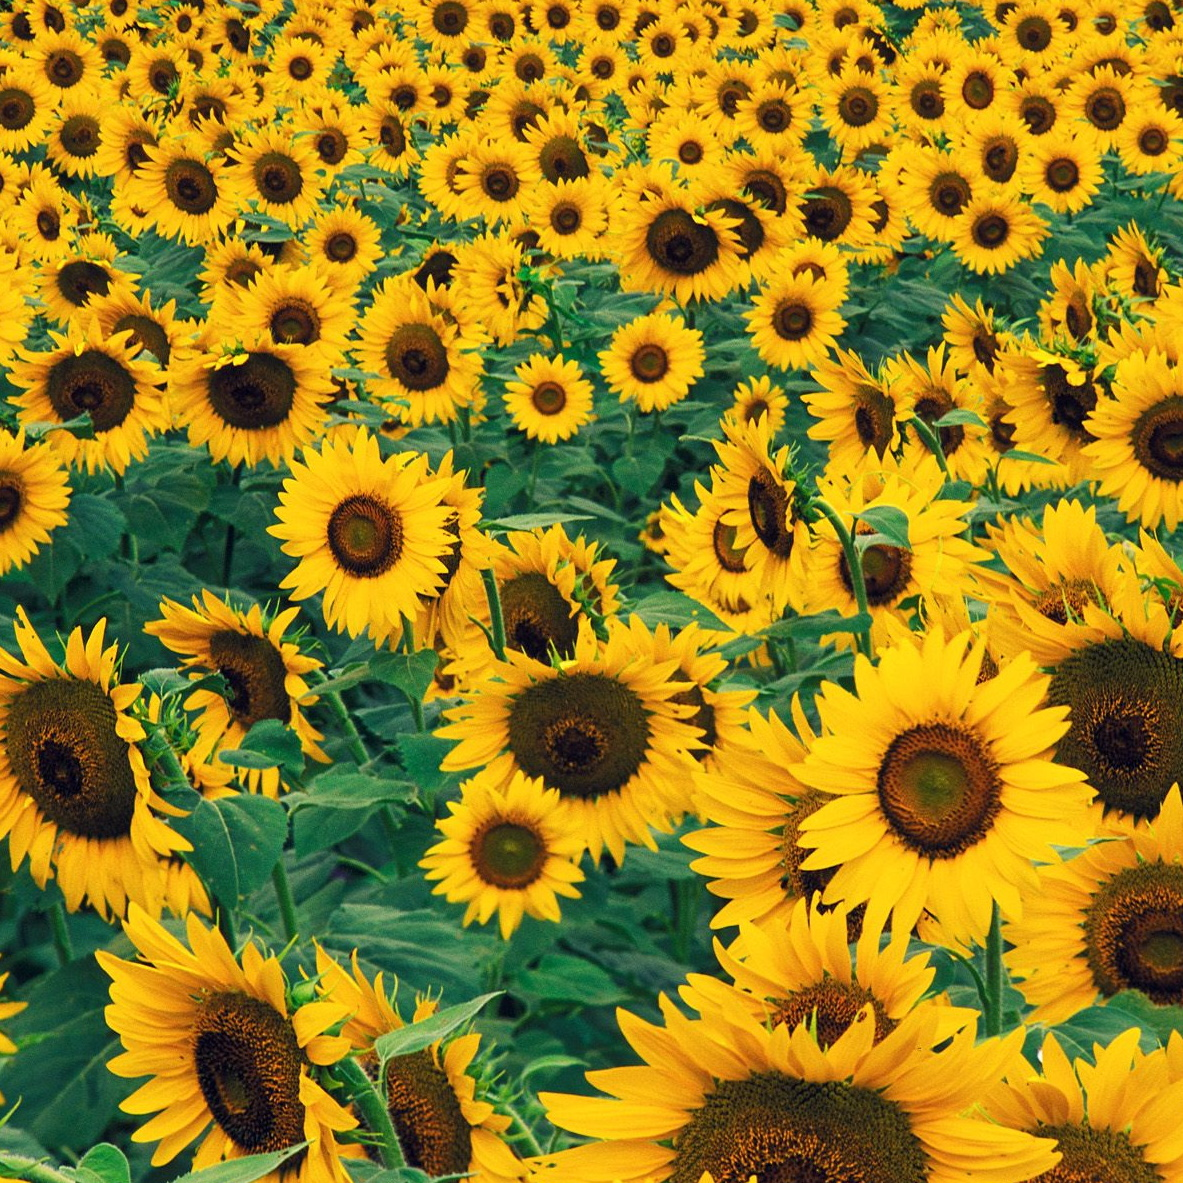
\includegraphics[height=1.5cm]{immagini/FF3.jpg}
	&Sara&Rizzo&59&Bologna&Fiorista\\
	\hline
	\cellcolor[HTML]{b0d7ff}\texttt{PF-7}&\cellcolor[HTML]{e6f2ff}\texttt{FF4}&	
	\vspace{.15cm}
	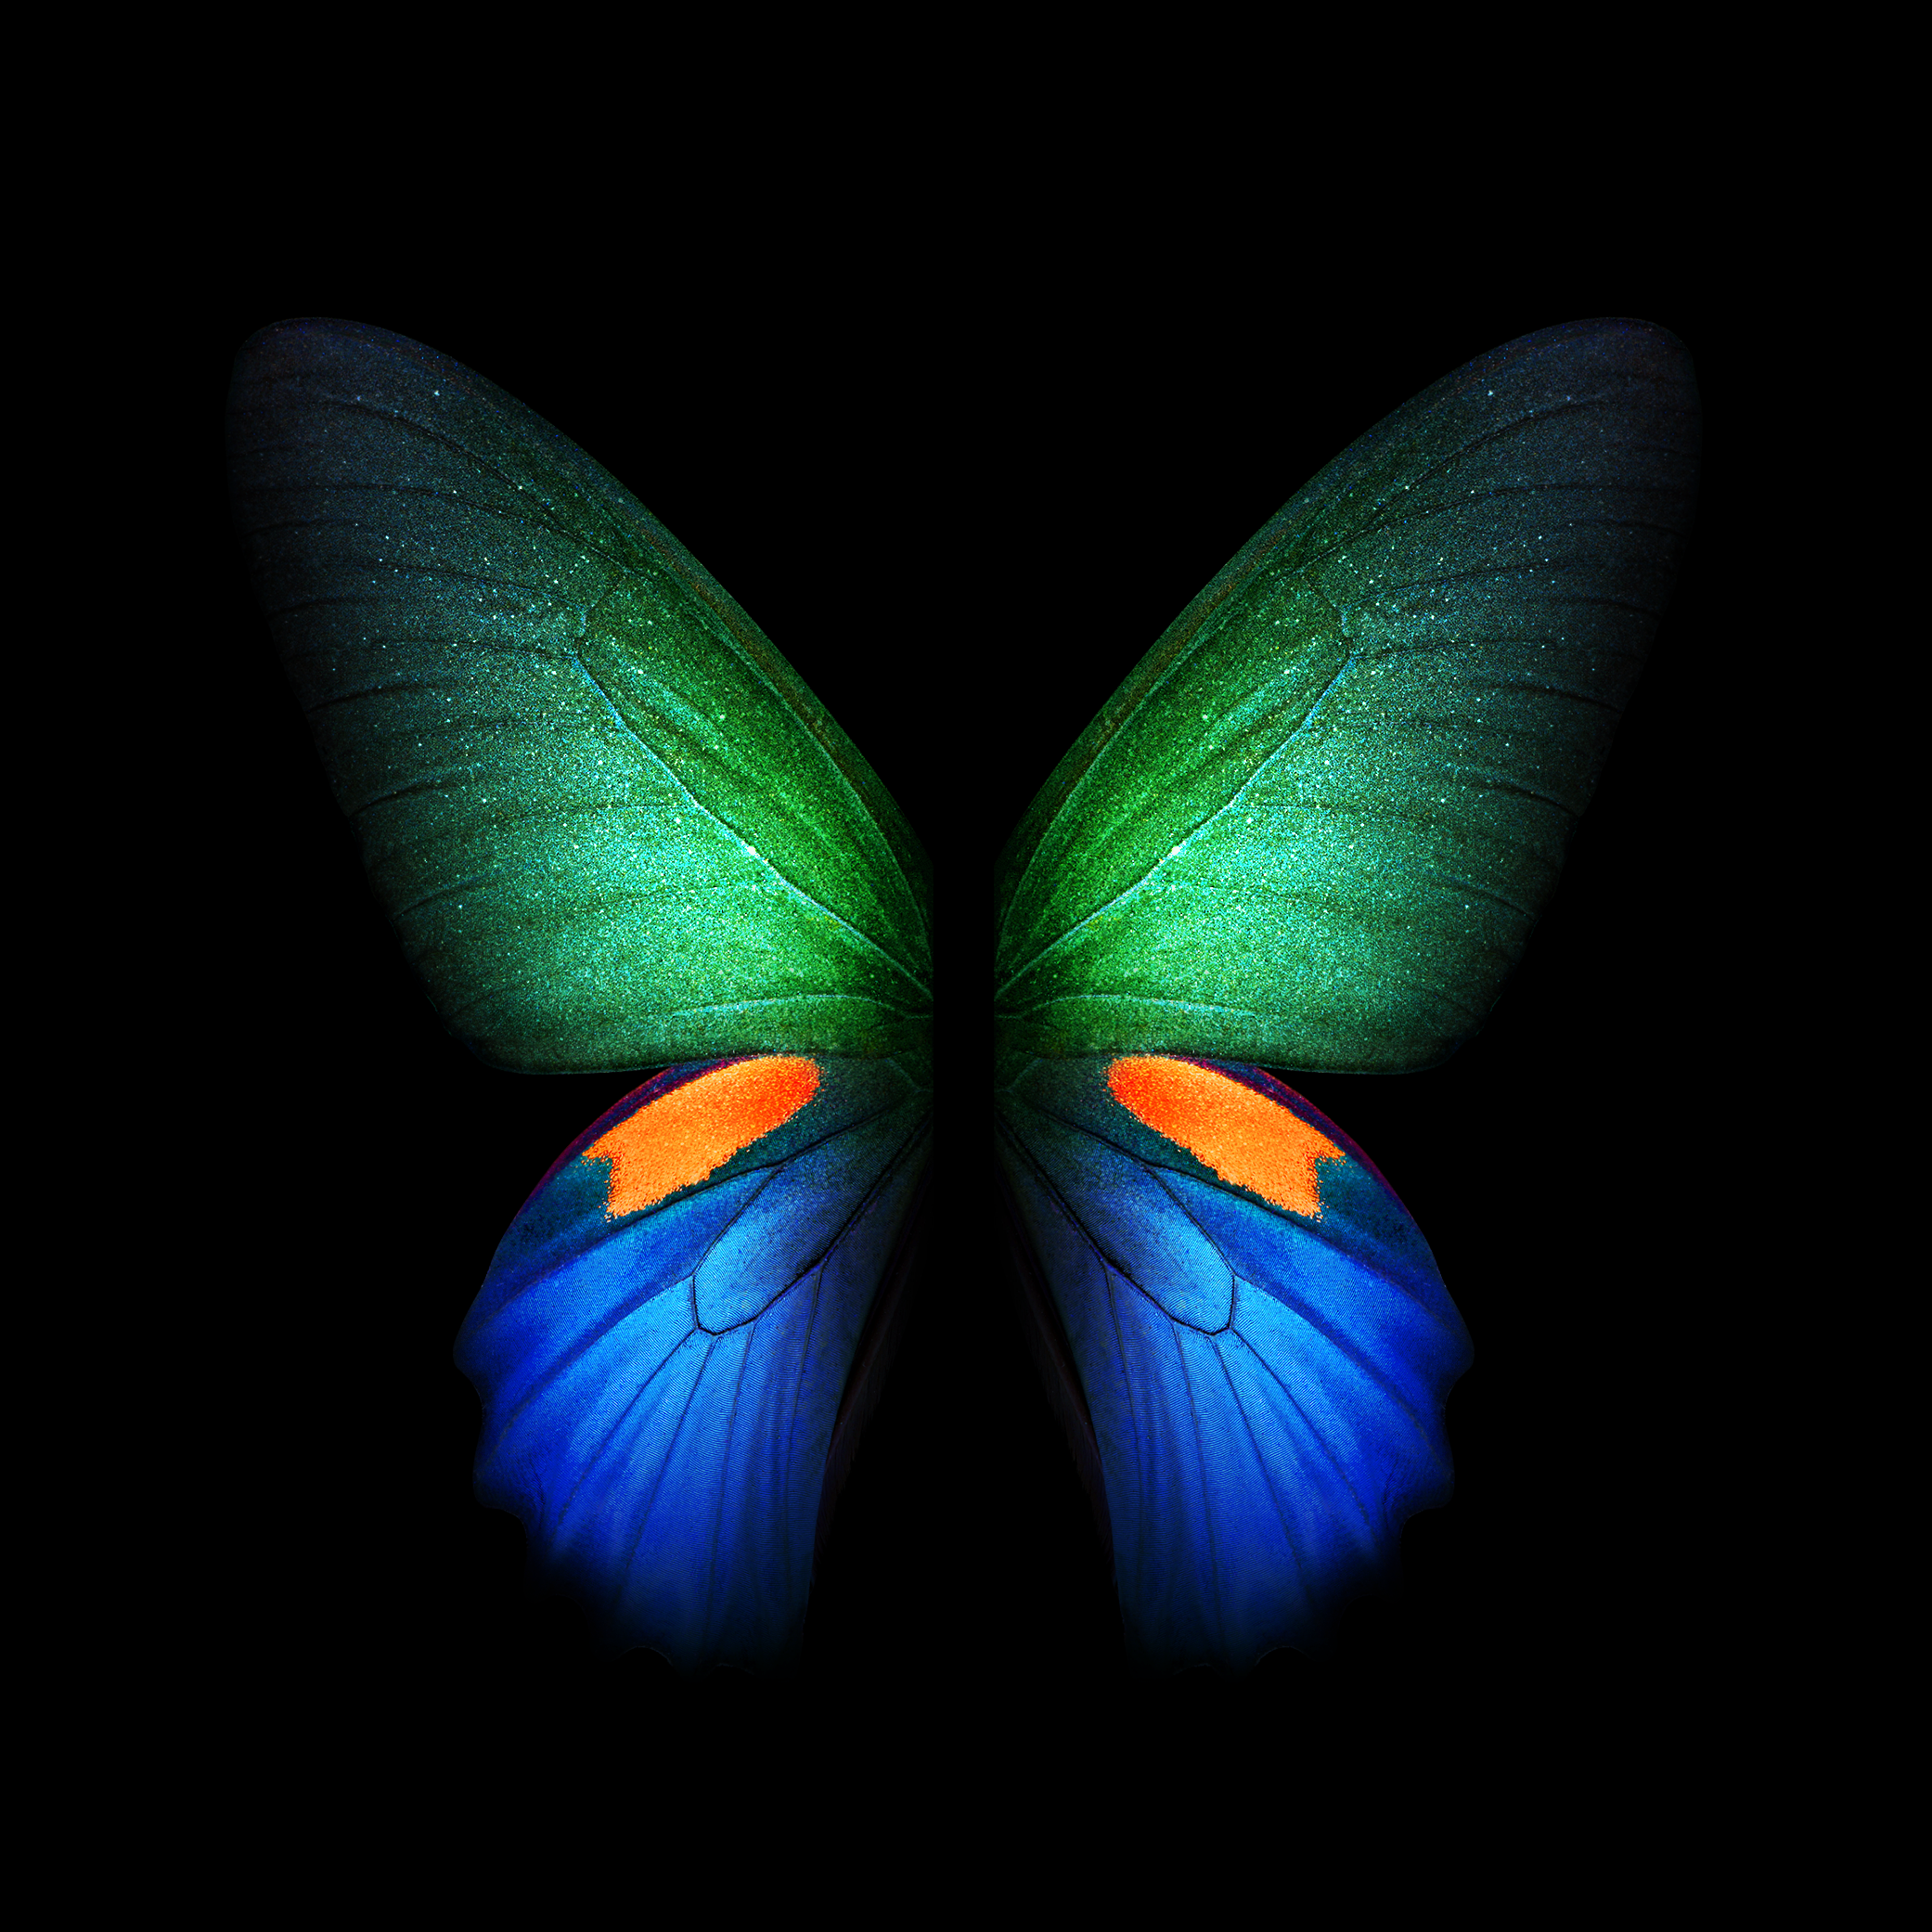
\includegraphics[height=1.5cm]{immagini/FF4.png}
	&Michela&D'Angelo&16&Taranto&Studentessa\\
	\hline 		
	\cellcolor[HTML]{b0d7ff}\texttt{PF-5}&\cellcolor[HTML]{e6f2ff}\texttt{MT2}&	
	\vspace{.15cm}
	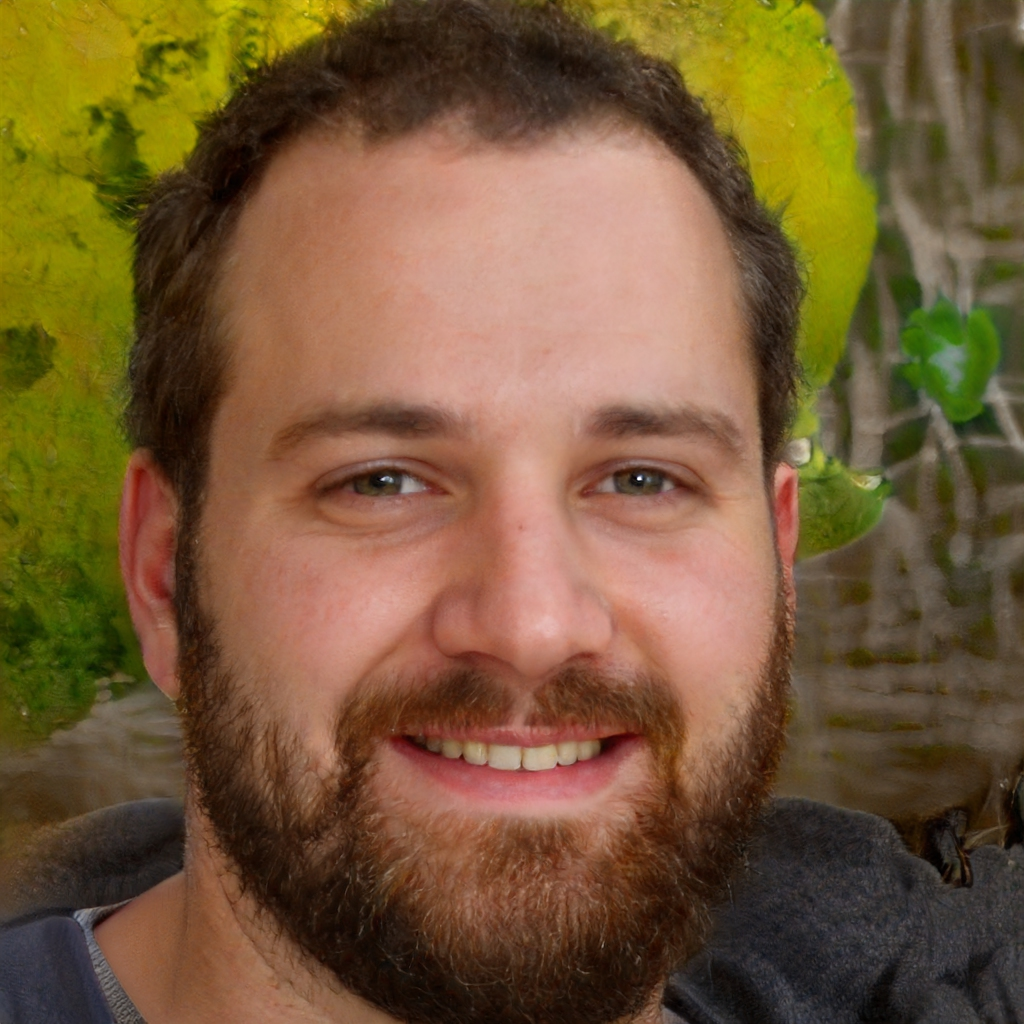
\includegraphics[height=1.5cm]{immagini/MT2.jpg}
	&Leonardo&Neri&45&Roma&Tatuatore\\
	\hline
	\cellcolor[HTML]{b0d7ff}\texttt{PF-3}&\cellcolor[HTML]{e6f2ff}\texttt{MT3}&	
	\vspace{.15cm}
	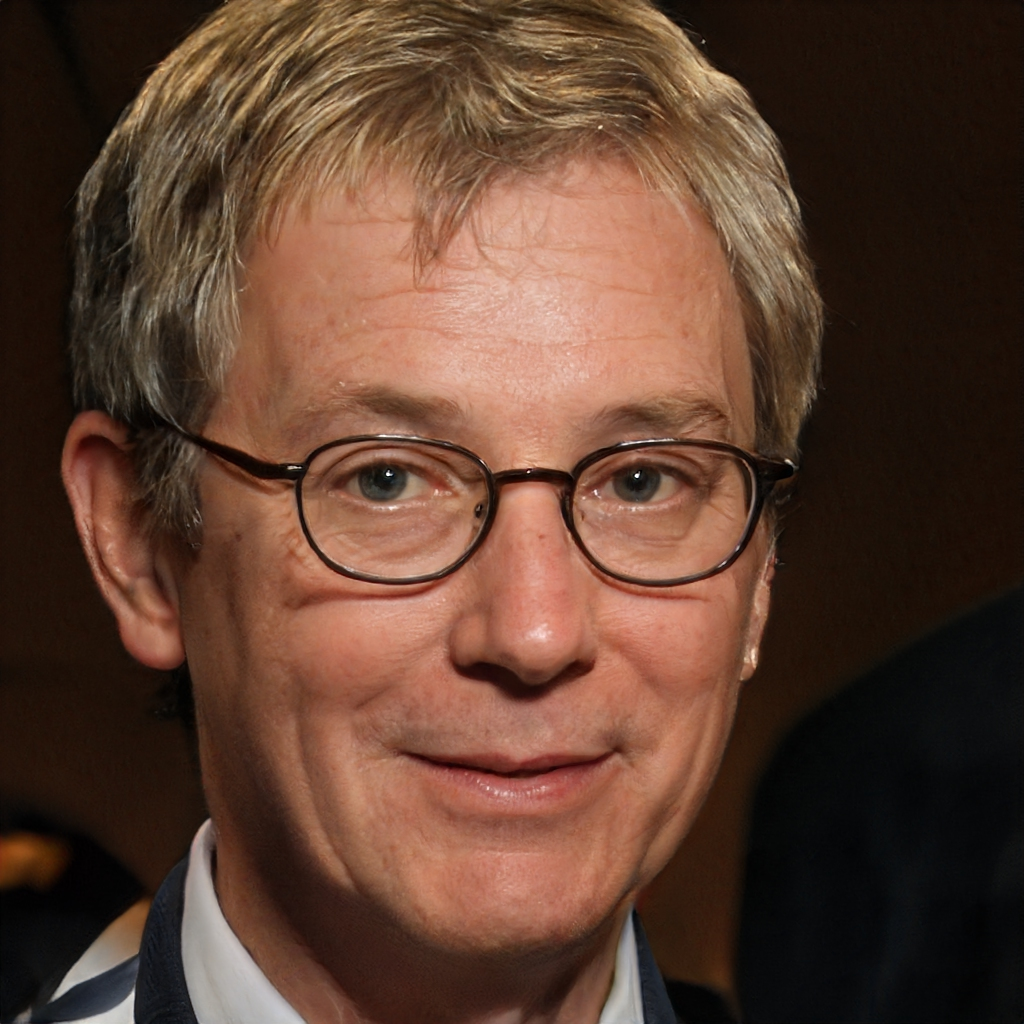
\includegraphics[height=1.5cm]{immagini/MT3.jpg}
	&Carlo&De Angelis&57&Siena&Chimico\\	 
	\hline
	\cellcolor[HTML]{b0d7ff}\texttt{PF-0}&\cellcolor[HTML]{e6f2ff}\texttt{MT4}&	
	\vspace{.15cm}
	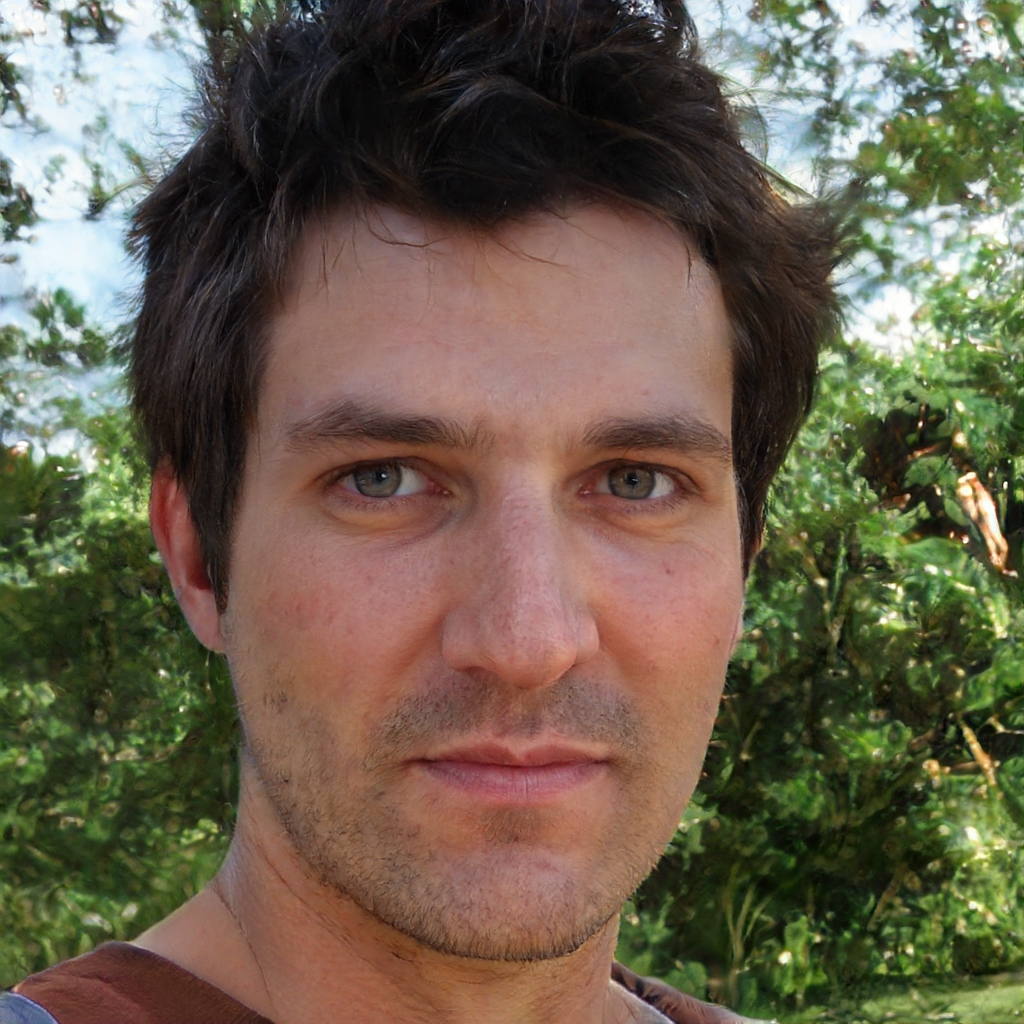
\includegraphics[height=1.5cm]{immagini/MT4.jpg}
	&Giuseppe&Martini&39&Ancona&Farmacista\\
	\hline
	\cellcolor[HTML]{b0d7ff}\texttt{PF-2}&\cellcolor[HTML]{e6f2ff}\texttt{MF2}&	
	\vspace{.15cm}
	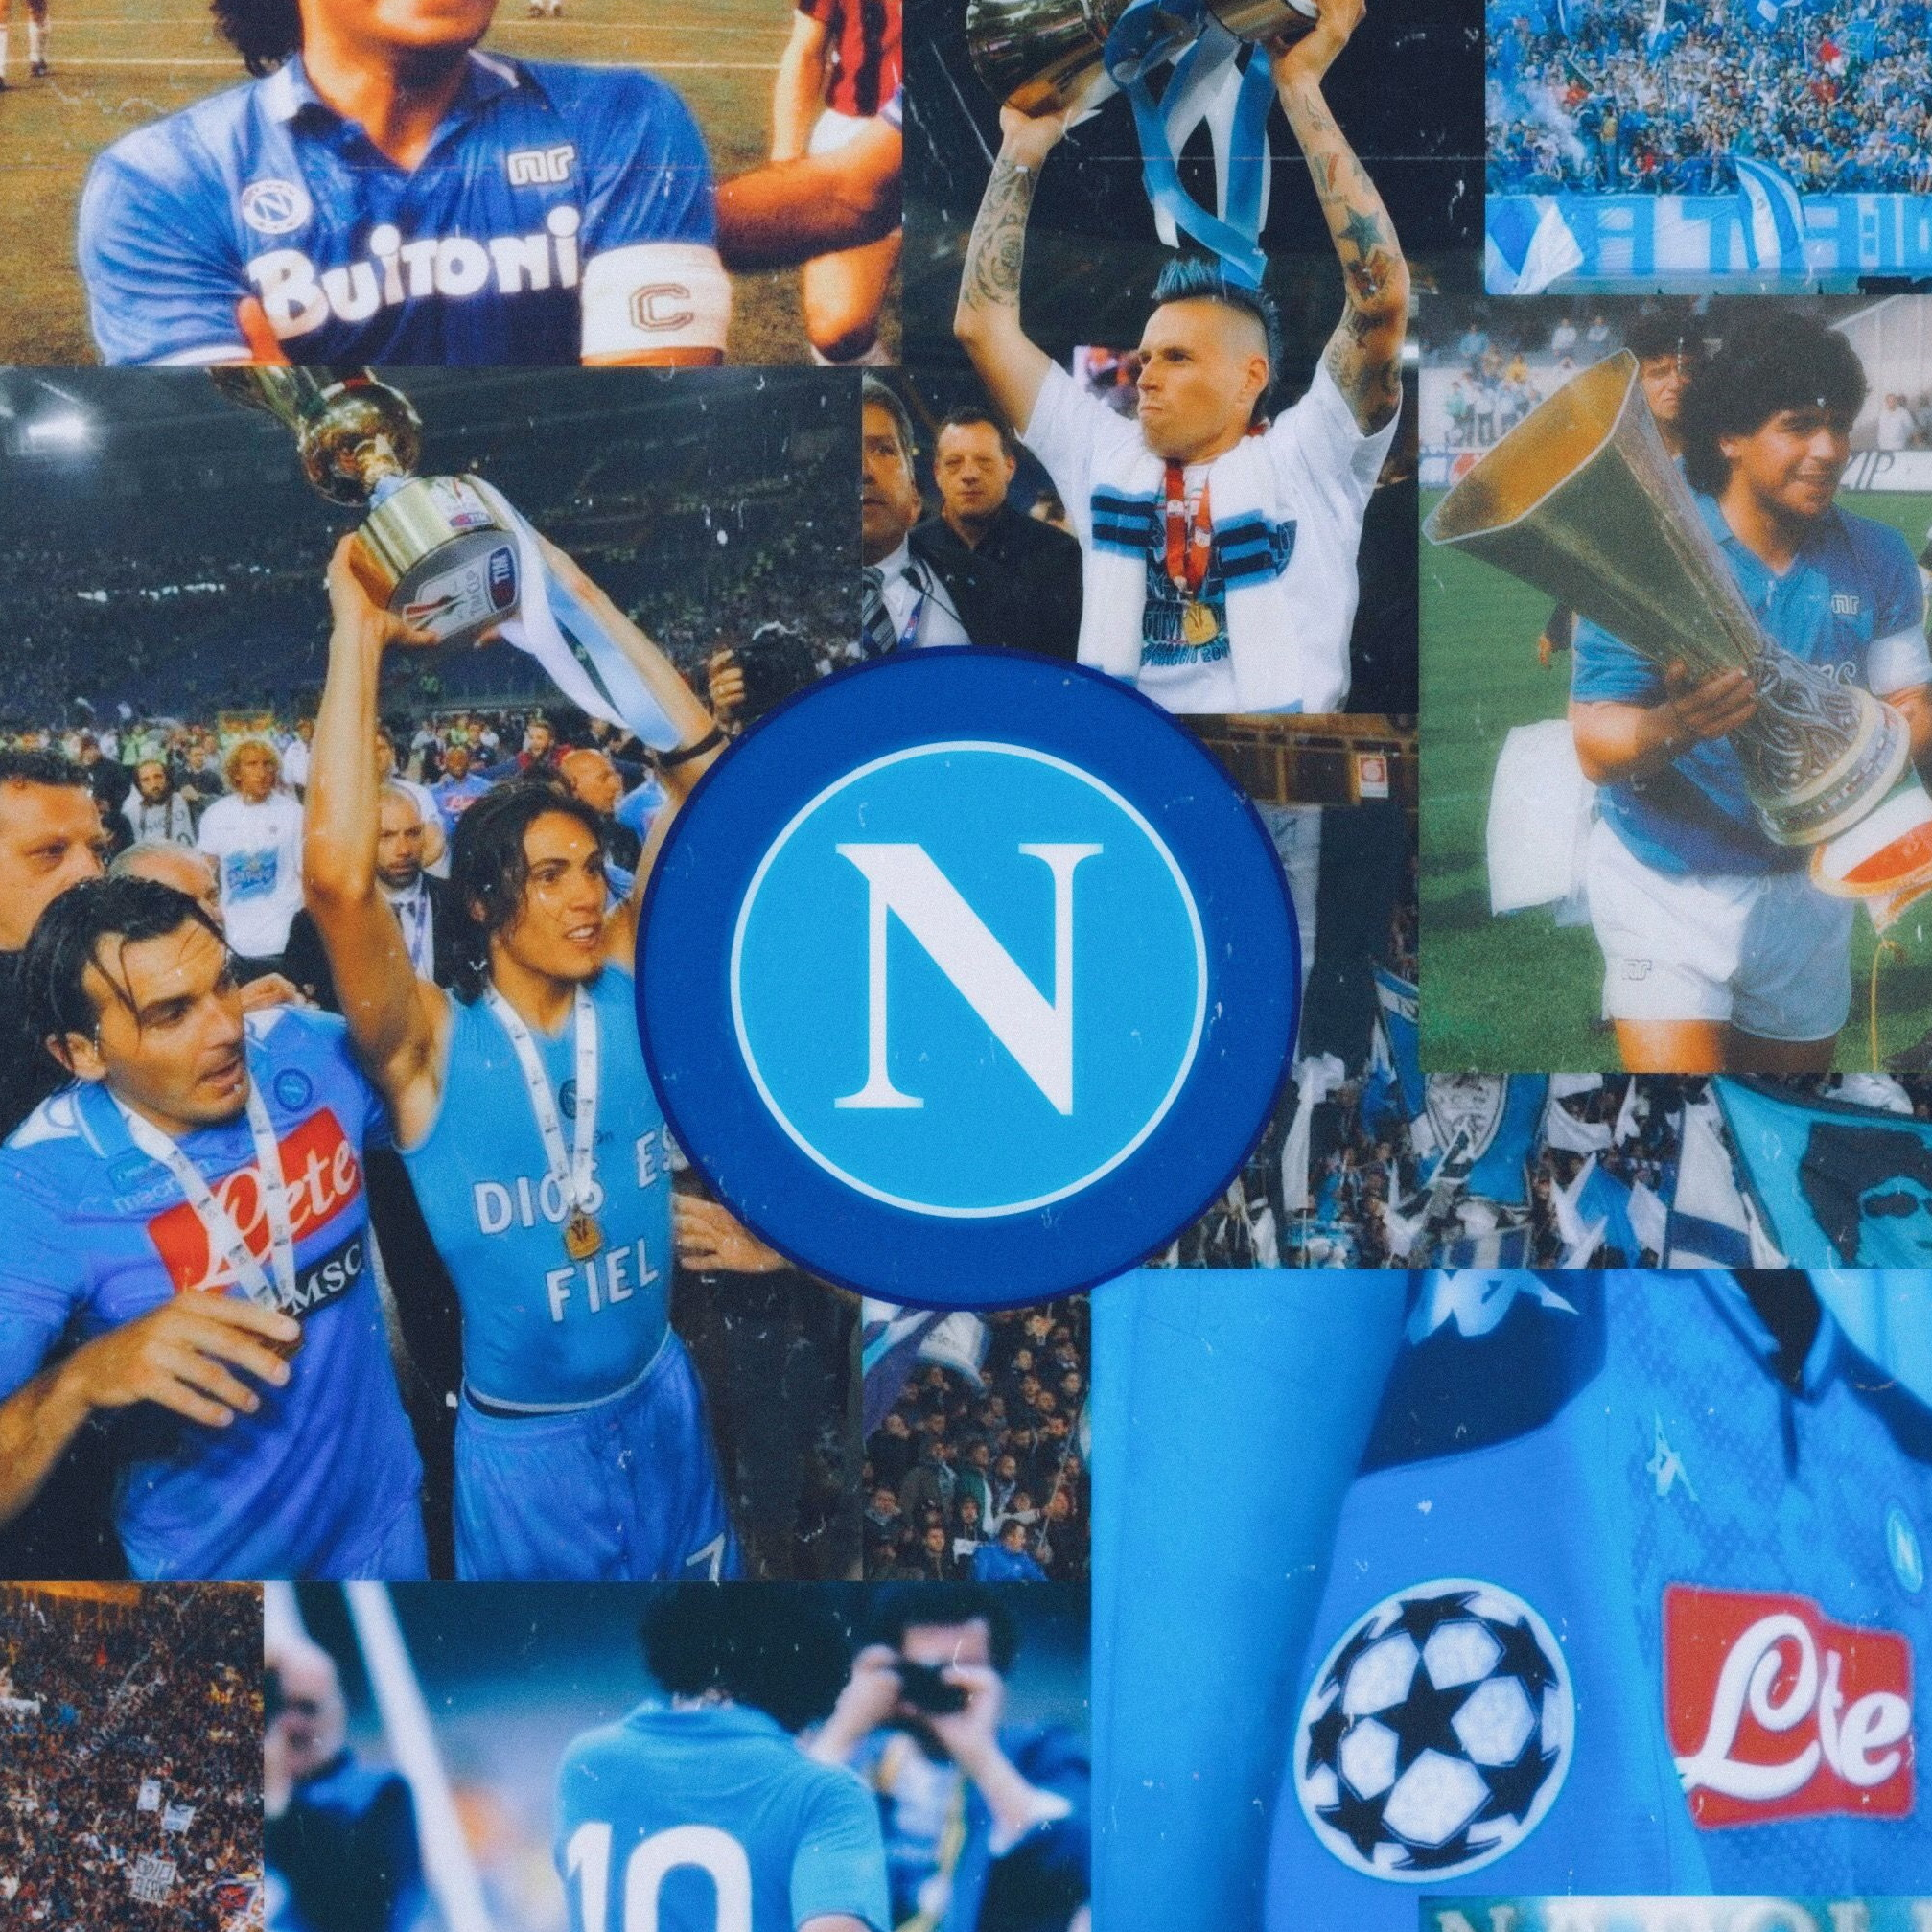
\includegraphics[height=1.5cm]{immagini/MF2.jpg}
	&Samuel&Colombo&44&Caserta&Tappezziere\\
	\hline
	\cellcolor[HTML]{b0d7ff}\texttt{PF-4}&\cellcolor[HTML]{e6f2ff}\texttt{MF3}&	
	\vspace{.15cm}
	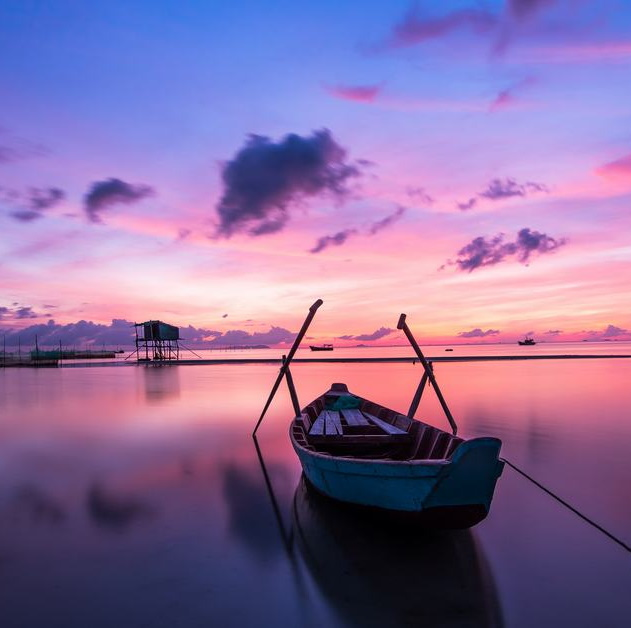
\includegraphics[height=1.5cm]{immagini/MF3.jpg}
	&Valerio&Mazza&57&Catanzaro&Dentista\\
	\hline
	\cellcolor[HTML]{b0d7ff}\texttt{PF-1}&\cellcolor[HTML]{e6f2ff}\texttt{MF4}&	
	\vspace{.15cm}
	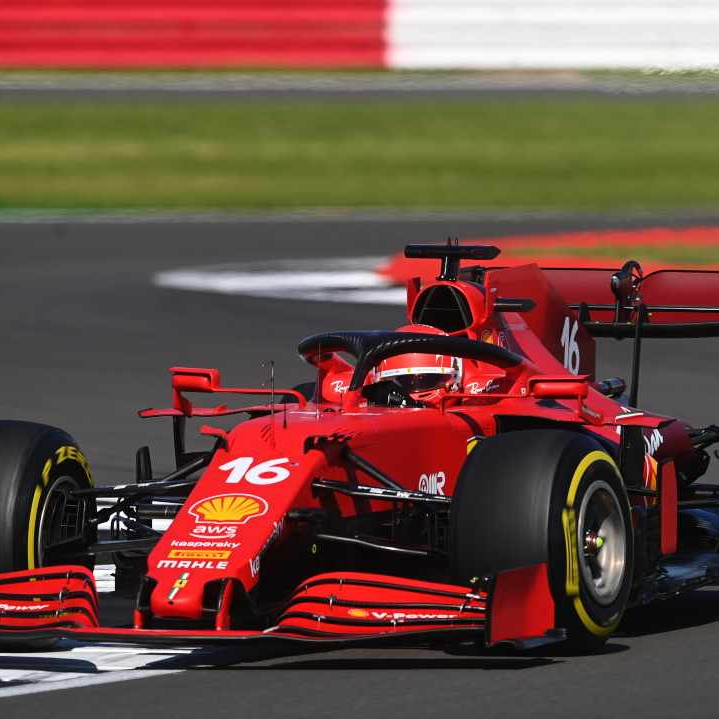
\includegraphics[height=1.5cm]{immagini/MF4.jpg}
	&Alessio&Fontana&17&Pescara&Studente\\
	\hline 	 	 	 	 	
\end{tabular}
\newpage
\section{Tool for automated search of a victim's profile}
This section reports the study and development process of the tool for searching for a victim profile in an automated way.\\\\
The initial idea was to develop a tool that would scrape and categorize the profiles at the same time they are searched for. 
\\For example, the tool logs into Facebook with the credentials of an attacker profile, somehow it gets a list of possible victim profiles and, one by one, it enters on it to scrape and categorize it, saving the result in the appropriate file. This means that the tool would move to the next profile until the list is over. \\
Computationally, this process is long and cumbersome, scraping would have increased significantly and, above all, this procedure is all done with a single attacker profile: this could be bring Facebook to block it, as it would always perform the same action in a loop for a long time.
\\\\Furthermore, the Facebook search interface is not helpful for this case study, as it gives the possibility to set the parameters of "city", "education", "work" and "friends of friends", and these parameters have nothing to do with this case study. \\\\
For all these reasons, it was necessary to proceed differently: first using a tool called \texttt{get-list-profile.py} to save a list of eligible victim profiles and then a subsequent tool called \texttt{classificator-profile.py} which determines for each profile if and what kind of victim it is.\\
The idea and operation of these two tools are now explained in detail.

\subsection{The tool: \texttt{get-list-profile.py}}
This first tool saves a list of profiles which will then be analyzed and classified by the next tool.
\\In detail, the tool, run from the terminal, requires as input:
\begin{itemize}
	\item \texttt{cod\_id}, that's the attacker's profile code;
	\item \texttt{type\_victim}, i.e. gender of the victim profiles that will be collect.\\Accepted values: string char $s$, with $s \in \{$\texttt{f, m}$\}$;.
\end{itemize}
First of all, the tool examine the attacker's \texttt{cod\_id} to verify that it exists and, if so, save its email and password to log in to Facebook. This is because it is not possible to search for profiles on Facebook without logging in.
\\\\At this point, based on the gender entered in the input, the tool randomly chooses a name from \texttt{dataset-names.json} and searches that name.
\\Facebook responds by showing a list of profiles with that name. But, more precisely, Facebook would show a list of profiles residing in a circumstantial area to that of the profile with which you are searching. To broaden the search range, we have chosen to use provinces instead of cities (and therefore to insert only the Italian provinces within the \texttt{dataset-city.json} dataset) and to disperse the attacker profiles throughout the Italian territory. 
\\\\Furthermore, each attacker profile searched for a minimum of 4 different named profiles with \texttt{gender = "f"} (i.e \textit{female}) and a minimum of 4 different named profiles with \texttt{gender = "m"} (i.e \textit{male}). A minimum or maximum limit was not given to the profiles to be collected, also because they were not yet assigned to the corresponding label.
\\\\In any case, from the list of resulting profiles, the tool clicks on the "Show all" button to load an even greater number of profiles and, scrolling the page a couple of times, saves in a \texttt{file} all user-profiles' url with the searched name.
\\\\Several copies of this tool have been created, which differ from each other for the file where they save the list of profiles. This was done to be able to work in parallel, in order to collect as many profiles as possible in the shortest possible time.

\subsection{The tool: \texttt{classificator-profile.py}}
\label{cap:classificator-profiles}
This second tool analyzes each profile of a given list (output of the previous tool) to be able to attach to each of them its corresponding label, and then save them in the appropriate dataset, called \texttt{victims.json}.
\\In detail, the tool, run from the terminal, requires as input:
\begin{itemize}
	\item \texttt{cod\_id}, that's the attacker's profile code;
	\item \texttt{file}, that's the name of the file containing the list of victim profiles that must be analyzed and categorized.
\end{itemize}
First of all, the tool examine the attacker's \texttt{cod\_id} to verify that it exists and, if so, save its email and password to log in to Facebook. This is because it is not possible to search for profiles on Facebook without logging in.
\\\\At this point, the tool opens the correct file based on the \texttt{file} parameter passed in input (the file is in the same folder as the tool).
It reads line by line, taking each URL that will lead to a saved victim profile.\\Once the URL has been selected, the tool moves to the dashboard of this profile, in order to analyze its details.
\\Here, the tool first checks for the presence of the button to add the profile to friends: some profiles do not allow you to be added to friends, but you can only follow them or send a private message. If the button is present, it will continue the analysis, otherwise, it will go to the next URL.
\\\\ As a first point, the tool checks the profile picture.
The algorithm uses the \texttt{alt} of the profile image to identify the presence (or not) of people within the image, a sufficient condition to make the \texttt{real\_img} parameter as \texttt{true} (details in chapter \ref{cap:alt-technology}).
\\Once it have checked the \texttt{alt} of the profile image, the tool will declare the image as "\texttt{T}" when the value of the "cod\_id" parameter is "true", otherwise it will declare "\texttt{F}".
\\\\After that, the tool will have to analyze what kind of URL the victim profile has. In fact, there are two types of profile URLs:
\begin{itemize}
	\item \texttt{https://www.facebook.com/profile.php?id=\textit{numerical\_sequence}}\\\textit{e.g. https://www.facebook.com/profile.php?id=3322661122}
	
	\item \texttt{https://www.facebook.com/\textit{character\_string}}\\(sometimes followed by \texttt{.\textit{numerical\_sequence}})\\\textit{e.g. https://www.facebook.com/mario.rossi.32}
\end{itemize}
Due to this difference, a check has been implemented to understand what type of URL you are dealing with and, consequently, the correct link is assigned to move within the profile to find the information.
\\\\At this point, the tool knows what type of URL it has to create for moving to the "about" page, where there is the basic information of the profile. 
\\\\Once here, thanks to a regular expression, the tool checks for the presence of a 4-character string, indicating the year of birth. If it is present, the age is calculated and the corresponding range between "2" or "3" is assigned, otherwise, the assigned range is "4" (details in chapter \ref{cap:age-parameter}).
\\\\As a last step, the tool analyzes the gender of the profile, first looking for the presence of the string "Man" or "Woman" and, if it is not found, it moves to \texttt{dataset-name.json} to search in which category that name is found. It will assign \texttt{F} if the profile is of a woman, \texttt{M} if it belongs to a man.
\\\\
Once at this point, the tool has created the corresponding label and this is where the \textit{check system} comes into play: before categorizing the profile, it asks for confirmation via the terminal, showing the label created. If it is correct, it's necessary to answer affirmative (with an "ok"), otherwise, the correct label must be enter.
\\Now, the tool has the exact label, so it can save the profile within the \texttt{victims.json} dataset, obviously after checking if that profile does not already exist.
\\\\Once the process is finished, move on to the next URL, until the list is over. Then, it destroys the \texttt{file} with the profile list and ends its execution.
\\\\A maximum limit for the profiles to have for each category has not been decided.\\On the contrary, a minimum number has been defined: each attacking profile will have to perform 3 friend requests for each category of victim profile (including the category in which it belongs). 
\\Considering that there are $12$ categories of attacker profiles, the minimum number of victim profiles for each category is $12 \cdot 3 = 36$ (so collect $12 \cdot 36 = 432$ victim profiles). An analysis tool aided this collection process, showing how many profiles were needed to reach the minimum value based on those already collected (details about the tool in chapter \ref{cap:victims-analysis}). 

\newpage
\section{Tool for automated friend request}
\label{cap:tool-friend-request}
This section reports the study and development process of the tool for the automated friend request from an attacker profile to one or more victim profiles.\\
This tool is the simplest in terms of implementation, as it was only necessary for it to log in and ask for friendship from a profile given in input. \\ 
But, considering that:
\begin{enumerate}
	\item each \textit{attacker} profile must send the friend request to 3 \textit{victim} profiles for each category;
	\item a \textit{victim} profile must not receive the friend request from more than one \textit{attacker} profile;
	\item each \textit{attacker} profile must have the same number of total friend requests to make;
	\item an \textit{attacker} profile mustn't send too many friend requests in close moments, because Facebook would block the profile.
\end{enumerate}
For this reason, first a tool called \texttt{round-add.py} was created and then the definitive friend request tool, called \texttt{add-friend.py}. 

\subsection{The tool: \texttt{round-add.py}}
This first tool must set the friendship requests that each \textit{attacker} profile has to send: it assigns to each attacker profile $36$ victim profiles to which to send the friend request. 
Each URL within the \texttt{victims.json} dataset is seen as an element of an array, and the name of the array is given by its category name.
\\ This tool must know:
\begin{itemize}
	\item the exact number of \textit{victim} profiles to witch each \textit{attacker} profile must send the friend request (36 in this case of study);
	\item the label of each \textit{victim} to witch one \textit{attacker} profile must send the friend request;
	\item the exact number of \textit{attacker} profile (12 in this case of study);
	\item the \texttt{cod} of each \textit{attacker} profile;
	\item the number of friend requests that each profile will have to send for each category (3 in this case of study).
\end{itemize}
The tool process this information and within the \texttt{set\_request.json} dataset, it will assign to each attacker profile the list of URLs of victim profiles to be attacked. It is nothing more than a list of positions of elements within each array containing the URL list of victim profiles. To calculate the index of each element, the numerical value of the \textit{attacker} profile is considered, to simulate a "jump" to the correct element, as many as there are attacker profiles available.\\
At this point, each attacking profile has its personal list of victim profiles to attack and the next tool comes into play.
\\\\ The tool, run from the terminal, doesn't need any input parameters:

\subsection{The tool: \texttt{add-friend.py}}
Given an attacker profile and its respective list of victim profiles that he will have to attack, this second tool takes care of requesting the friendship from the \textit{attacker} profile to the \textit{victim} profile.\\
Hovwever to avoid being blocked by Facebook, it was decided to structure this attack in rounds: at each round, identified with an index, an attacker profile will have to send the friend request from \texttt{n} victim profiles.\\
The tool point to the first element of the victim profiles list of one specific attacker profile, skipping the elements that are part of the previous rounds.
\\There is a list that specifies how many friend request must be sent in every round (values ranging from 1 friend request to 4 friend requests). The index of each elements of this list is the identification value of the round.\\\\
For example, at the 3rd round, knowing the number of profiles to which must request friendship in the previous rounds, the sum of them point to the first element of the victim profiles list to which the current attacker profile must send the friend request in this round.
\\In detail, the tool, run from the terminal, requires as input:
\begin{itemize}
	\item \texttt{cod\_id}, that's the attacker's profile code;
	\item \texttt{round}, the numerical value that indicates the attack round to be satisfied.
\end{itemize}
At this point, each \textit{attacker} profile will log into Facebook and send the friend requests to the victim profiles taken from the correct portion of the list in that particular round. \\
To manage this delicate phase more accurately, an excel file has been built to keep track of the rounds already executed.
\\Once the friend request has been sent to a \textit{victim} profile, before moving on to the next one, the tool saves the information in a dataset called \texttt{request\_log.json}: for each attacker profile, the list of attacked victim profiles are indicated, with its specific category.             % Product Design Freeze e SOP
% !TEX encoding = UTF-8
% !TEX TS-program = pdflatex
% !TEX root = ../tesi.tex

%**************************************************************
\chapter{Data collection}
\label{cap:data-collection}
In this chapter all the developed analysis tools will be explained. For data collection, it wouldn't have been required to develop special tools.
\par \noindent Nevertheless, they have been implemented because they are useful and, above all, usable even in contexts where the amount of data collected is considerably greater. Moreover, it was preferred to develop separate tools that perform individual analysis functions. This was done thinking about the fact that these tools could also be used individually in the future in contexts where it will not be necessary to follow a chronological order of execution every time.
\par \noindent In addition, a \textit{time control system} has been developed: the analysis tools also keep track of the date on which they are performed to make visible the trend over time because some victim profiles may accept the friend request later because they previously kept it suspended.
\par \noindent
Each result of each analysis session is enclosed in a folder named with the date on which the analysis session was carried out.

%**************************************************************
\section{Analyze victims: \texttt{victims-analysis.py} tool}
\label{cap:victims-analysis}
To determine the evolution of the \texttt {victims.json} dataset growth during the execution of the tool named \texttt {classificator-profile.py} (details in Chapter \ref{cap:classificator-profiles}), it was created a simple tool, called \texttt{victims-analysis.py}. \par \noindent This tool show on the terminal how many profiles for each category of victim profiles have been saved up to then in the \texttt{victims.json} dataset.
\par \noindent Furthermore, to make distribution more intuitive, it shows (but not save) a bar graph that highlights the difference in the victim profiles collected for each category.
\par \noindent This tool was very useful during the execution of the \texttt{classificator-profile.py} tool because it allowed to keep under constant control the trend of the dataset, and, above all, to be able to check that every category will reach the minimum value. 
\par \noindent From this tool, it was possible to observe that the dataset is heavily \textit{unbalanced} (detail in Chapter \ref{cap:discuss-dataset-victims}).

\section{Analyze outcomes of friend requests}
After sending all the friend requests with each attacker profile (details in Chapter \ref{cap:friend-request-sent}), we started to launch these various analysis tools.
To do this as automatically as possible, a series of tools have been created, each based on its specific functionality.
\par \noindent The developed tools are:
\begin{enumerate}
	\item \texttt{cleaning-save-distribution.py};
	\item \texttt{analyze-friend-requests.py};
	\item \texttt{get-distribution.py};
	\item \texttt{report-acceptance.py}.
\end{enumerate}
These tools must be run in exactly this order each time. Now they will be explain.
\subsection{The tool: \texttt{clean-save-distribution-contents.py}}
This first simple tool cleans the contents of the \texttt{save\_distribution.json}, i.e., it will set its each value to 0. Considering that these tools must be run one after the other on each analysis session, this particular tool must be run first because it modifies the starting file for the analysis. If it contains data from previous analysis sessions, it is invalid because the data would overlap. So, with this tool, the content of this dataset is cleaned up as if it had just been created and therefore ready to accept the new data for a new analysis session.\par \noindent 
Although the function is small, this mini tool was created separately, as it could be used at any time (for example if some error occurs during the analysis). Potentially, this tool could also be run only at the end of each analysis session. The important thing is that every time a new analysis session begins, \texttt{save\_distribution.json} dataset must be cleaned.

\subsection{The tool: \texttt{analyze-friend-requests.py}}
This tool verifies for each attacker profile which of the victim profiles has accepted the friend request. Using a list with all the identification codes of the attacker profiles, it fetch the information necessary to log in on Facebook and then it save the list of friends' URLs in a temporary file. A function will read the temporary file line by line and find a match with a URL in the \texttt{request-log.json} file in the section dedicated to the attacker profile under consideration. For each profile found, will increase the count inside the \texttt{save\_distribution.json} file, so that at the end of the analysis of each attacker profile, it is possible to see, for each victim, how many and what type of profiles attackers accepted the friend request.\par \noindent 
In the end, It also will show in the terminal how many friend requests have been accepted out of the total of those sent.

\subsection{The tool: \texttt{get-distribution.py}}
\label{cap:distribution-update}
This tool shows the distribution of the friend requests accepted: for each victim, it creates a graph that displays how many friend requests the victim accepted and from which attacker profiles they came from. The tool will first create a folder called ``report'' with the date the tool is started (for example ``report-2021-08-02''). Then, inside it will save bar graphs that show this information. Each image contains a graphic about a specific victim and is saved with today's date and victim type (for example ``2021-08-02 - 7-MT3''). Furthermore, it creates \texttt{distribution\_}\textit{current\_date}\texttt{.json} dataset and update the content of \texttt{distribution\_update.json} dataset, with the report of the data in \texttt{JSON} struct. They are the same file, but the first one is useful to see the report during the time, the last one will be use to have the last updated data to create the \textit{model of acceptance} (details in \ref{cap:model-of-acceptance}). 

\subsection{The tool: \texttt{report-acceptance.py}}
\label{cap:tool-report-acc}
The last tool to run, called ``\texttt{report-acceptance.py}'', focuses on the attacker who made the friend request. First of all, it creates a folder called \texttt{''report-request''} where it saves a bar chart for each attacker profile showing, for each category of victim profile, how many requests have been made by that attacker profile. In this case study, it would not be necessary considering that there are 3 friend requests for each victim profile, but if you have to work with more data this function will be needed again. Then, it will create a second folder, called ``\texttt{report-acceptance}'', where it saves a bar chart for each attacker profile, showing, for each category of victim profile, how many requests have been accepted to that attacker profile. It will also save this information in the \texttt{distribution\_data} file where \emph{data} means the date the tool was executed (for example ``\texttt{distribution\_2021-08-02}'').
             % Conclusioni
\appendix                               
% !TEX encoding = UTF-8
% !TEX TS-program = pdflatex
% !TEX root = ../tesi.tex

%**************************************************************
\chapter{Appendice A}
%**************************************************************

\epigraph{Citazione}{Autore della citazione}



             % Appendice A

%**************************************************************
% Materiale finale
%**************************************************************
\backmatter
\printglossaries
% !TEX encoding = UTF-8
% !TEX TS-program = pdflatex
% !TEX root = ../tesi.tex

%**************************************************************
% Bibliografia
%**************************************************************

\cleardoublepage
\chapter{Bibliography}

\nocite{*}
% Stampa i riferimenti bibliografici
%\printbibliography[heading=subbibliography,title={Riferimenti bibliografici},type=book]

% Stampa i siti web consultati
\printbibliography[heading=subbibliography,title={References},type=online]


\end{document}
